%% bare_jrnl.tex
%% V1.4b
%% 2015/08/26
%% by Michael Shell
%% see http://www.michaelshell.org/
%% for current contact information.
%%
%% This is a skeleton file demonstrating the use of IEEEtran.cls
%% (requires IEEEtran.cls version 1.8b or later) with an IEEE
%% journal paper.
%%
%% Support sites:
%% http://www.michaelshell.org/tex/ieeetran/
%% http://www.ctan.org/pkg/ieeetran
%% and
%% http://www.ieee.org/

%%*************************************************************************
%% Legal Notice:
%% This code is offered as-is without any warranty either expressed or
%% implied; without even the implied warranty of MERCHANTABILITY or
%% FITNESS FOR A PARTICULAR PURPOSE! 
%% User assumes all risk.
%% In no event shall the IEEE or any contributor to this code be liable for
%% any damages or losses, including, but not limited to, incidental,
%% consequential, or any other damages, resulting from the use or misuse
%% of any information contained here.
%%
%% All comments are the opinions of their respective authors and are not
%% necessarily endorsed by the IEEE.
%%
%% This work is distributed under the LaTeX Project Public License (LPPL)
%% ( http://www.latex-project.org/ ) version 1.3, and may be freely used,
%% distributed and modified. A copy of the LPPL, version 1.3, is included
%% in the base LaTeX documentation of all distributions of LaTeX released
%% 2003/12/01 or later.
%% Retain all contribution notices and credits.
%% ** Modified files should be clearly indicated as such, including  **
%% ** renaming them and changing author support contact information. **
%%*************************************************************************


% *** Authors should verify (and, if needed, correct) their LaTeX system  ***
% *** with the testflow diagnostic prior to trusting their LaTeX platform ***
% *** with production work. The IEEE's font choices and paper sizes can   ***
% *** trigger bugs that do not appear when using other class files.       ***                          ***
% The testflow support page is at:
% http://www.michaelshell.org/tex/testflow/



\documentclass[journal]{IEEEtran}
%
% If IEEEtran.cls has not been installed into the LaTeX system files,
% manually specify the path to it like:
% \documentclass[journal]{../sty/IEEEtran}





% Some very useful LaTeX packages include:
% (uncomment the ones you want to load)


% *** MISC UTILITY PACKAGES ***
%
%\usepackage{ifpdf}
% Heiko Oberdiek's ifpdf.sty is very useful if you need conditional
% compilation based on whether the output is pdf or dvi.
% usage:
% \ifpdf
%   % pdf code
% \else
%   % dvi code
% \fi
% The latest version of ifpdf.sty can be obtained from:
% http://www.ctan.org/pkg/ifpdf
% Also, note that IEEEtran.cls V1.7 and later provides a builtin
% \ifCLASSINFOpdf conditional that works the same way.
% When switching from latex to pdflatex and vice-versa, the compiler may
% have to be run twice to clear warning/error messages.






% *** CITATION PACKAGES ***
%
%\usepackage{cite}
% cite.sty was written by Donald Arseneau
% V1.6 and later of IEEEtran pre-defines the format of the cite.sty package
% \cite{} output to follow that of the IEEE. Loading the cite package will
% result in citation numbers being automatically sorted and properly
% "compressed/ranged". e.g., [1], [9], [2], [7], [5], [6] without using
% cite.sty will become [1], [2], [5]--[7], [9] using cite.sty. cite.sty's
% \cite will automatically add leading space, if needed. Use cite.sty's
% noadjust option (cite.sty V3.8 and later) if you want to turn this off
% such as if a citation ever needs to be enclosed in parenthesis.
% cite.sty is already installed on most LaTeX systems. Be sure and use
% version 5.0 (2009-03-20) and later if using hyperref.sty.
% The latest version can be obtained at:
% http://www.ctan.org/pkg/cite
% The documentation is contained in the cite.sty file itself.






% *** GRAPHICS RELATED PACKAGES ***
%
\ifCLASSINFOpdf
  % \usepackage[pdftex]{graphicx}
  % declare the path(s) where your graphic files are
  % \graphicspath{{../pdf/}{../jpeg/}}
  % and their extensions so you won't have to specify these with
  % every instance of \includegraphics
  % \DeclareGraphicsExtensions{.pdf,.jpeg,.png}
\else
  % or other class option (dvipsone, dvipdf, if not using dvips). graphicx
  % will default to the driver specified in the system graphics.cfg if no
  % driver is specified.
  % \usepackage[dvips]{graphicx}
  % declare the path(s) where your graphic files are
  % \graphicspath{{../eps/}}
  % and their extensions so you won't have to specify these with
  % every instance of \includegraphics
  % \DeclareGraphicsExtensions{.eps}
\fi
% graphicx was written by David Carlisle and Sebastian Rahtz. It is
% required if you want graphics, photos, etc. graphicx.sty is already
% installed on most LaTeX systems. The latest version and documentation
% can be obtained at: 
% http://www.ctan.org/pkg/graphicx
% Another good source of documentation is "Using Imported Graphics in
% LaTeX2e" by Keith Reckdahl which can be found at:
% http://www.ctan.org/pkg/epslatex
%
% latex, and pdflatex in dvi mode, support graphics in encapsulated
% postscript (.eps) format. pdflatex in pdf mode supports graphics
% in .pdf, .jpeg, .png and .mps (metapost) formats. Users should ensure
% that all non-photo figures use a vector format (.eps, .pdf, .mps) and
% not a bitmapped formats (.jpeg, .png). The IEEE frowns on bitmapped formats
% which can result in "jaggedy"/blurry rendering of lines and letters as
% well as large increases in file sizes.
%
% You can find documentation about the pdfTeX application at:
% http://www.tug.org/applications/pdftex





% *** MATH PACKAGES ***
%
%\usepackage{amsmath}
% A popular package from the American Mathematical Society that provides
% many useful and powerful commands for dealing with mathematics.
%
% Note that the amsmath package sets \interdisplaylinepenalty to 10000
% thus preventing page breaks from occurring within multiline equations. Use:
%\interdisplaylinepenalty=2500
% after loading amsmath to restore such page breaks as IEEEtran.cls normally
% does. amsmath.sty is already installed on most LaTeX systems. The latest
% version and documentation can be obtained at:
% http://www.ctan.org/pkg/amsmath





% *** SPECIALIZED LIST PACKAGES ***
%
%\usepackage{algorithmic}
% algorithmic.sty was written by Peter Williams and Rogerio Brito.
% This package provides an algorithmic environment fo describing algorithms.
% You can use the algorithmic environment in-text or within a figure
% environment to provide for a floating algorithm. Do NOT use the algorithm
% floating environment provided by algorithm.sty (by the same authors) or
% algorithm2e.sty (by Christophe Fiorio) as the IEEE does not use dedicated
% algorithm float types and packages that provide these will not provide
% correct IEEE style captions. The latest version and documentation of
% algorithmic.sty can be obtained at:
% http://www.ctan.org/pkg/algorithms
% Also of interest may be the (relatively newer and more customizable)
% algorithmicx.sty package by Szasz Janos:
% http://www.ctan.org/pkg/algorithmicx




% *** ALIGNMENT PACKAGES ***
%
%\usepackage{array}
% Frank Mittelbach's and David Carlisle's array.sty patches and improves
% the standard LaTeX2e array and tabular environments to provide better
% appearance and additional user controls. As the default LaTeX2e table
% generation code is lacking to the point of almost being broken with
% respect to the quality of the end results, all users are strongly
% advised to use an enhanced (at the very least that provided by array.sty)
% set of table tools. array.sty is already installed on most systems. The
% latest version and documentation can be obtained at:
% http://www.ctan.org/pkg/array


% IEEEtran contains the IEEEeqnarray family of commands that can be used to
% generate multiline equations as well as matrices, tables, etc., of high
% quality.




% *** SUBFIGURE PACKAGES ***
%\ifCLASSOPTIONcompsoc
%  \usepackage[caption=false,font=normalsize,labelfont=sf,textfont=sf]{subfig}
%\else
%  \usepackage[caption=false,font=footnotesize]{subfig}
%\fi
% subfig.sty, written by Steven Douglas Cochran, is the modern replacement
% for subfigure.sty, the latter of which is no longer maintained and is
% incompatible with some LaTeX packages including fixltx2e. However,
% subfig.sty requires and automatically loads Axel Sommerfeldt's caption.sty
% which will override IEEEtran.cls' handling of captions and this will result
% in non-IEEE style figure/table captions. To prevent this problem, be sure
% and invoke subfig.sty's "caption=false" package option (available since
% subfig.sty version 1.3, 2005/06/28) as this is will preserve IEEEtran.cls
% handling of captions.
% Note that the Computer Society format requires a larger sans serif font
% than the serif footnote size font used in traditional IEEE formatting
% and thus the need to invoke different subfig.sty package options depending
% on whether compsoc mode has been enabled.
%
% The latest version and documentation of subfig.sty can be obtained at:
% http://www.ctan.org/pkg/subfig




% *** FLOAT PACKAGES ***
%
%\usepackage{fixltx2e}
% fixltx2e, the successor to the earlier fix2col.sty, was written by
% Frank Mittelbach and David Carlisle. This package corrects a few problems
% in the LaTeX2e kernel, the most notable of which is that in current
% LaTeX2e releases, the ordering of single and double column floats is not
% guaranteed to be preserved. Thus, an unpatched LaTeX2e can allow a
% single column figure to be placed prior to an earlier double column
% figure.
% Be aware that LaTeX2e kernels dated 2015 and later have fixltx2e.sty's
% corrections already built into the system in which case a warning will
% be issued if an attempt is made to load fixltx2e.sty as it is no longer
% needed.
% The latest version and documentation can be found at:
% http://www.ctan.org/pkg/fixltx2e


%\usepackage{stfloats}
% stfloats.sty was written by Sigitas Tolusis. This package gives LaTeX2e
% the ability to do double column floats at the bottom of the page as well
% as the top. (e.g., "\begin{figure*}[!b]" is not normally possible in
% LaTeX2e). It also provides a command:
%\fnbelowfloat
% to enable the placement of footnotes below bottom floats (the standard
% LaTeX2e kernel puts them above bottom floats). This is an invasive package
% which rewrites many portions of the LaTeX2e float routines. It may not work
% with other packages that modify the LaTeX2e float routines. The latest
% version and documentation can be obtained at:
% http://www.ctan.org/pkg/stfloats
% Do not use the stfloats baselinefloat ability as the IEEE does not allow
% \baselineskip to stretch. Authors submitting work to the IEEE should note
% that the IEEE rarely uses double column equations and that authors should try
% to avoid such use. Do not be tempted to use the cuted.sty or midfloat.sty
% packages (also by Sigitas Tolusis) as the IEEE does not format its papers in
% such ways.
% Do not attempt to use stfloats with fixltx2e as they are incompatible.
% Instead, use Morten Hogholm'a dblfloatfix which combines the features
% of both fixltx2e and stfloats:
%
% \usepackage{dblfloatfix}
% The latest version can be found at:
% http://www.ctan.org/pkg/dblfloatfix




%\ifCLASSOPTIONcaptionsoff
%  \usepackage[nomarkers]{endfloat}
% \let\MYoriglatexcaption\caption
% \renewcommand{\caption}[2][\relax]{\MYoriglatexcaption[#2]{#2}}
%\fi
% endfloat.sty was written by James Darrell McCauley, Jeff Goldberg and 
% Axel Sommerfeldt. This package may be useful when used in conjunction with 
% IEEEtran.cls'  captionsoff option. Some IEEE journals/societies require that
% submissions have lists of figures/tables at the end of the paper and that
% figures/tables without any captions are placed on a page by themselves at
% the end of the document. If needed, the draftcls IEEEtran class option or
% \CLASSINPUTbaselinestretch interface can be used to increase the line
% spacing as well. Be sure and use the nomarkers option of endfloat to
% prevent endfloat from "marking" where the figures would have been placed
% in the text. The two hack lines of code above are a slight modification of
% that suggested by in the endfloat docs (section 8.4.1) to ensure that
% the full captions always appear in the list of figures/tables - even if
% the user used the short optional argument of \caption[]{}.
% IEEE papers do not typically make use of \caption[]'s optional argument,
% so this should not be an issue. A similar trick can be used to disable
% captions of packages such as subfig.sty that lack options to turn off
% the subcaptions:
% For subfig.sty:
% \let\MYorigsubfloat\subfloat
% \renewcommand{\subfloat}[2][\relax]{\MYorigsubfloat[]{#2}}
% However, the above trick will not work if both optional arguments of
% the \subfloat command are used. Furthermore, there needs to be a
% description of each subfigure *somewhere* and endfloat does not add
% subfigure captions to its list of figures. Thus, the best approach is to
% avoid the use of subfigure captions (many IEEE journals avoid them anyway)
% and instead reference/explain all the subfigures within the main caption.
% The latest version of endfloat.sty and its documentation can obtained at:
% http://www.ctan.org/pkg/endfloat
%
% The IEEEtran \ifCLASSOPTIONcaptionsoff conditional can also be used
% later in the document, say, to conditionally put the References on a 
% page by themselves.




% *** PDF, URL AND HYPERLINK PACKAGES ***
%
%\usepackage{url}
% url.sty was written by Donald Arseneau. It provides better support for
% handling and breaking URLs. url.sty is already installed on most LaTeX
% systems. The latest version and documentation can be obtained at:
% http://www.ctan.org/pkg/url
% Basically, \url{my_url_here}.




% *** Do not adjust lengths that control margins, column widths, etc. ***
% *** Do not use packages that alter fonts (such as pslatex).         ***
% There should be no need to do such things with IEEEtran.cls V1.6 and later.
% (Unless specifically asked to do so by the journal or conference you plan
% to submit to, of course. )


% correct bad hyphenation here
\hyphenation{op-tical net-works semi-conduc-tor}

\usepackage{amsmath,amssymb,amsthm}
\usepackage{xparse}
\usepackage{latexsym}
\usepackage{amsfonts}
\usepackage{graphicx}
\usepackage{txfonts}
\usepackage{wasysym}
\usepackage{enumitem}
\usepackage{adjustbox}
\usepackage{ragged2e}
\usepackage{tabularx}
\usepackage{changepage}
\usepackage{setspace}
\usepackage{hhline}
\usepackage{multicol}
\usepackage{float}
\usepackage{multirow}
\usepackage{makecell}
\usepackage{fancyhdr}
\usepackage[toc,page]{appendix}
\usepackage[utf8]{inputenc}
\usepackage[T1]{fontenc}
\usepackage{hyperref}
\usepackage{isomath}
\usepackage{fixmath}
\usepackage{tikz}
\usepackage{textcomp}
\usepackage{epstopdf} %converting to PDF
\usepackage{upgreek}
\usepackage{mathtools}
\usepackage{xfrac}
\usepackage{lipsum}
\usepackage[colorinlistoftodos]{todonotes}
\input{./Modules/LatexShortcuts_Itayyeka_2.tex}
%%%%%%%%%%%%%%    aliases    %%%%%%%%%%%%%%
\newcommand{\dTheta}{\Delta\theta}
\newcommand{\dTau}{\Delta\tau}
\newcommand{\D}[2]{\mathcal{D}\left(#1,#2\right)}
\newcommand{\Dp}[3]{\mathcal{D}^{#3}\left(#1,#2\right)}
\newcommand{\fbBpRatio}{
\left|
\frac{
\frac
{
\vecnot{\alpha}^{T}\vecnot{d}_{\theta_{s}}exp\left(-j\tau_{s}\right)
}
{
4c^{2}\tau_{s}^{2}-\vecnot{\beta}^{T}\vecnot{d}_{\theta_{s}}exp\left(-j\tau_{s}\right)
}
}{
\frac
{
\vecnot{\alpha}^{T}\vecnot{d}_{\theta}exp\left(-j\tau\right)
}
{
4c^{2}\tau^{2}-\vecnot{\beta}^{T}\vecnot{d}_{\theta}exp\left(-j\tau\right)
}
}
\right|
}
\newcommand{\Hr}[3]{\mathcal{H}^{#3}\left(#1,#2\right)}
\newcommand{\Steer}[1]{\vecnot{d}_{#1}}

\NewDocumentCommand{\evalat}{sO{\big}mm}{%
  \IfBooleanTF{#1}
   {\mleft. #3 \mright|_{#4}}
   {#3#2|_{#4}}%
}

\newcommand{\hDen}{\left(4c^{2}\tau^{2}-\vecnot{\beta}^{T}\vecnot{d}e^{-j\omega\tau}\right)}
%%%%%%%%%%%%%%%%%%%%%%%%%%%%%%%%%%%%%%%%%%%%%%%%%%%%%%
%%%%%%%%%%%%%%      Document flags     %%%%%%%%%%%%%%%
%%%%%%%%%%%%%%%%%%%%%%%%%%%%%%%%%%%%%%%%%%%%%%%%%%%%%%
% \def\showDev{}
\def\DEFIncludeAttenuation
%%%%%%%%%%%%  Document Code starts here %%%%%%%%%%%%%%

\begin{document}
%
% paper title
% Titles are generally capitalized except for words such as a, an, and, as,
% at, but, by, for, in, nor, of, on, or, the, to and up, which are usually
% not capitalized unless they are the first or last word of the title.
% Linebreaks \\ can be used within to get better formatting as desired.
% Do not put math or special symbols in the title.
\title{Novel approach to beamforming.\\Localization with spatial feedback.}
%
%
% author names and IEEE memberships
% note positions of commas and nonbreaking spaces ( ~ ) LaTeX will not break
% a structure at a ~ so this keeps an author's name from being broken across
% two lines.
% use \thanks{} to gain access to the first footnote area
% a separate \thanks must be used for each paragraph as LaTeX2e's \thanks
% was not built to handle multiple paragraphs
%

\author{Itay Yehezkel Karo,~\IEEEmembership{Non Member,~IEEE,}
        Tsvi G. Dvorkind,~\IEEEmembership{Non Member,~IEEE,}
        Israel Cohen,~\IEEEmembership{Fellow,~IEEE}
\thanks{I. Y. Karo and I. Cohen are with the departement of EE, Technion.}% <-this % stops a space
\thanks{T. G. Dvorkind is with Rafael corp.}% <-this % stops a space
}

% note the % following the last \IEEEmembership and also \thanks - 
% these prevent an unwanted space from occurring between the last author name
% and the end of the author line. i.e., if you had this:
% 
% \author{....lastname \thanks{...} \thanks{...} }
%                     ^------------^------------^----Do not want these spaces!
%
% a space would be appended to the last name and could cause every name on that
% line to be shifted left slightly. This is one of those "LaTeX things". For
% instance, "\textbf{A} \textbf{B}" will typeset as "A B" not "AB". To get
% "AB" then you have to do: "\textbf{A}\textbf{B}"
% \thanks is no different in this regard, so shield the last } of each \thanks
% that ends a line with a % and do not let a space in before the next \thanks.
% Spaces after \IEEEmembership other than the last one are OK (and needed) as
% you are supposed to have spaces between the names. For what it is worth,
% this is a minor point as most people would not even notice if the said evil
% space somehow managed to creep in.



% The paper headers
\markboth{IEEE tran. sig. proc.}%
{Karo \MakeLowercase{\textit{et al.}}: Beamforming with feedback}
% The only time the second header will appear is for the odd numbered pages
% after the title page when using the twoside option.
% 
% *** Note that you probably will NOT want to include the author's ***
% *** name in the headers of peer review papers.                   ***
% You can use \ifCLASSOPTIONpeerreview for conditional compilation here if
% you desire.




% If you want to put a publisher's ID mark on the page you can do it like
% this:
%\IEEEpubid{0000--0000/00\$00.00~\copyright~2015 IEEE}
% Remember, if you use this you must call \IEEEpubidadjcol in the second
% column for its text to clear the IEEEpubid mark.



% use for special paper notices
%\IEEEspecialpapernotice{(Invited Paper)}




% make the title area
\maketitle

% As a general rule, do not put math, special symbols or citations
% in the abstract or keywords.
\begin{abstract}
A new feedback based approach for array signal processing is suggested. In the proposed scheme, a signal is continuously re-transmitted between the array and the target of interest. We analyze this system in the context of beamforming for source localization and show a significant improvement in several key features, such as reducing the obtained beam-width, increasing its peak to side-lobe level and improving the array directivity. 
\end{abstract}

% Note that keywords are not normally used for peerreview papers.
\begin{IEEEkeywords}
Spatial array processing, localization, beam-pattern.
\end{IEEEkeywords}






% For peer review papers, you can put extra information on the cover
% page as needed:
% \ifCLASSOPTIONpeerreview
% \begin{center} \bfseries EDICS Category: 3-BBND \end{center}
% \fi
%
% For peerreview papers, this IEEEtran command inserts a page break and
% creates the second title. It will be ignored for other modes.
\IEEEpeerreviewmaketitle
% The very first letter is a 2 line initial drop letter followed
% by the rest of the first word in caps.
% 
% form to use if the first word consists of a single letter:
% \IEEEPARstart{A}{demo} file is ....
% 
% form to use if you need the single drop letter followed by
% normal text (unknown if ever used by the IEEE):
% \IEEEPARstart{A}{}demo file is ....
% 
% Some journals put the first two words in caps:
% \IEEEPARstart{T}{his demo} file is ....
% 
% Here we have the typical use of a "T" for an initial drop letter
% and "HIS" in caps to complete the first word.
\section{Introduction}
\IEEEPARstart{T}{he} 
general field of array processing has been thoroughly studied in many contexts throughout several decades, producing many important application such as spatial filtering, source localization, signal detection, source separation, manifold learning, feature extraction, and many more.
Spatial sensor arrays enable the extraction of spatial information such as localizing a transmitting source \cite{skolnik2008radar} \myTodo{inline}{\textbf{DONE:}\\cite some radar book}, blindly separating mixtures of impinging signals \cite{Comon1994IndependentConcept} \myTodo{inline}{\textbf{DONE:}\\here you can cite some papers which talk about BSS and ICA signal source separation. Make sure to cite something which is well known, that is, has many citations}, improving signal to noise ratio (SNR) \myTodo{inline}{\textbf{DONE:}\\cite some works/books about MVDR,MPDR processing}\cite{Frost1972AProcessing,verdu1998multiuser} and many more. 
\par Uniform linear array (ULA), a uniformly spaced structure of sensors, has always been a point of interest, due to its simplicity of analysis \cite{VanTrees2002DetectionIV}. 
The array size and the number of its elements $N$ has significant influence on the obtained array performance, such as SNR improvement, spatial separation capabilities and its number of degrees of freedom (DOF). For example, the influential MUSIC algorithm \cite{Ralph1986MultipleParameter} enables to detect up to $N-1$ directions of arrival (DOA) due to $N-1$ spatially separated sources, by projecting the possible steering vectors (SV) of the array manifold onto the noise subspace.
The limitation on the number of processed or detected sources due to the limited amount of DOF of a given array, inspired different directions of research.\myTodo{inline}{\textbf{ACCEPTED:}\\you are focusing on the DOF problem, but this is not the main focus of our paper...} 
\par One approach, involving different array geometries, examined minimum redundancy arrays \cite{Moffet1968Minimum-RedundancyArrays,Pillai1985AEstimation,UnnikrishnaPillai1987StatisticalMatrix} \myTodo{inline}{are those the works were we look at arrays with 'holes' and fill in the void due to second order statistics across the existing elements?\\\textbf{ANSWER}\\ No, those works deal with non-uniform linear arrays, reducing the element spacing redundancy, such that for $N$ element array, there will be the minimal number of pair with a specific difference. The main purpose is to increase resolution by reducing ambiguity. The extraction of the "holes" is the "virtual array" concept which is mentioned next} trying to reduce the spatial ambiguity through minimization of redundant inter-element spacing in order to increase the overall resolution. 
\par Another approach, commonly referenced as ``virtual arrays" \cite{Pal2010NestedFreedom,Chevalier2005OnProcessing,Mendel1999ApplicationsProcessing}\myTodo{inline}{are you citing known works? \\\textbf{(Yes, for example \cite{Chevalier2005OnProcessing} is cited ~200 times)}\\ I think Veydanathan \\\textbf{ADDED his work.}\\(hope that spelling correctly) did some works on this. Also Arye Yeredor from TAU} deals with the extraction of samples originated in sensors that do not really exist (i.e. relying on higher order statistics and manipulating multiple statistical cross-terms in order to estimate statistical characteristics of signals impinging in missing sensors). 
Using a similar approach, the $2q$-MUSIC algorithm \cite{Chevalier2006High-resolutionAlgorithm} \myTodo{inline}{not familiar... \\\textbf{Has around ~140 citations}\\}, enables the use of $N^{2q}$ ``virtual elements'', by calculating the $q$'th order statistics. \myTodo{inline}{\textbf{REPHRASED: and reduced}\\did not understand this last sentence. You did not explain what are nested arrays.}
\par A well known \cite{VanVeenBeamforming:Filtering} equivalence, which inspired the current paper, is the analogy between ULA spatial array processing of narrow-band signals and finite impulse response (FIR) temporal filtering. 
In the context of temporal signal processing, it is well known that for a given filter order $N$, in many cases, the infinite impulse response (IIR) filter leads to improved performance, as compared to FIR filter design of the same order. In particular, narrow transition regions, and low sidelobes can be achieved by implementing feedback based filtering. 
\par This naturally arises the question, ``what are the equivalent spatial domain processing methods which will be analogous to temporal IIR filtering? " 
\par A related work \cite{Wen2013ExtendingStructure} has also addressed this question. 
There, in the context of ULA, two approaches were considered. \myTodo{inline}{\textbf{DONE:}\\The next sentence is not clear. Please rephrase}
The first one was to estimate the time of arrival (TOA) difference between two consecutive sensors and to synthetically generate the recursive part of the IIR filter, entirely in the time-domain. 
The second approach suggested to consider overlapping subsets of one large ULA as finite approximation to an infinite array. Surely, the former approach heavily relies on the accuracy of the delay estimation and the latter approach does not achieve a recursive spatial response. In both cases, there is no true spatial feedback between the array and the source of interest.
\par Other works \cite{Madanayake2008AFilters,Madanayake2008ABeamformer} use the concept of $2D$ spatio-temporal plane wave representation (i.e. a straight line angled according to the DOA in the spatio-temporal plane), to design ultra-wide-band (UWB) filters \cite{L.Bruton1983HighlyPlanes} which both sample spatial snapshots of the signal and recursively process it in temporal domain. \myTodo{inline} {\textbf{REPHRASED}\\please explain (maybe later just to me) how UWB filtering is used}\myTodo{inline}{\textbf{Removed - not important - a way of implementation}\\what is that?}\myTodo{inline}{\textbf{DONE:}\\what are the drawbacks if these last papers?}
Here as well, the recursive part of the filter is obtained entirely in the temporal domain.  
\par The goal in this contribution, is to present a sensor array processing approach which achieves spatial-domain feedback-based processing, similarly to IIR filtering in the time domain. Opposed the previous works, we do not wish to estimate the inter-element delay and apply the recursive part in the time domain, but rather implement the feedback entirely in the spatial domain.
We focus on a localization problem, where our goal is to estimate the direction and the range of some target.
Opposed to classical array processing, we incorporate spatial feedback, show its equivalence to IIR filtering in case of a ULA, and analyze some key aspects of the proposed scheme. 

The spatial feedback between the array and the target is created by constantly re-transmitting a signal and its echoes between the array and the target. 
The initial stimulus can be generated at the target itself or at the location of the array. In the text to follow, we assume this is the latter. 

Also, similar to radar applications, the target can be passive and merely reflect the impinging signal, or to be cooperative, i.e. by receiving, enhancing the signal and re-transmitting it back to the array. In this work, we assume the former.

\par The outline of this paper is as follows. We first formulate the classic spatial beamforming setup in Sec.~\ref{sec:setup}. Then, in Sec.~\ref{sec_introduceFeedback}, we propose our novel feedback based architecture, and calculate its spatial response. In Sec.~ \ref{sec_FIM} we evaluate the Fisher Information Matrix (FIM) and discuss optimal choices of the array weights in order to  maximize the information in detecting the target's range and DOA. In Sec.~\ref{sec_Performance} we evaluate some key features of the proposed beamforming with feedback. Specifically, we compute the array beamwidth, its peak to sidelobe ratio and the array directivity, showing significant improvement compared to traditional beamforming without spatial feedback. 
In Sec.~\ref{sec_app} we simulate the proposed processing scheme, and emphasis its sensitivity to range errors. We then suggest a strategy which eliminates this sensitivity. Finally, concluding remarks are stated in Sec.~\ref{sec_conclusions}.
\myTodo{inline}{Here you should state the content of the paper. In Sec. \ref{sec:setup} we define our setup. In Sec. ... we analyze the suggested feedback based system. etc...}
\section{Classical Beamforming }\label{sec:setup}
\myTodo{inline}{\textbf{DONE:}\\ why to speak only about ULA? The work is more general and ULA is a special case. Will rephrase this whole section}Consider an $N$-element array with $n$'th sensor at position $p_n,\; n=0,\ldots,N-1$, where we define $p_{0}=0$ to be the reference point for future analysis. Let $p_t$ be the position of a target of interest. We focus on a far field localization problem, aiming for DOA and target range estimation. Without loss of generality, and for simplicity of the exposition, we reduce the discussion to a 2D problem, denoting the DOA by a single angle $\theta_g$. The range $R$ between the array and the target of interest can be computed with respect to some reference sensor, say $p_{0}$, i.e. $R\triangleq\norm{p_{t}-p_{0}}$. 
Inspired by radar based applications, we assume that the signal $x(t)$ is transmitted from the array, reflects back from the target and re-impinges the array, with total time delay of $\tau_{pd}=2R/c$ seconds, where $c$ represents the propagation velocity of the signal in the medium. Opposed to radar applications, we assume that the target of interest is static. 

Let $x_{n,\theta_g}(t)$ be the measured signal at the $n$'th sensor of the array
\begin{equation}
x_{n,\theta_g}(t) = g_{n,\theta_{g}}x\Brack{t-\tau_{pd}-\tau_{n,\theta_{g}}},
\label{eqn:noFeedbackULA_singleSensor_temporal}
\end{equation}
where $g_{n,\theta_{g}}$ represents the gain due to medium attenuation, the influence of target's radar cross section (RCS) and the sensor's gain at DOA $\theta_g$. Here, $\tau_{n,\theta_{g}}$ represents the arrival time difference of the signal between the $n$'th sensor (at $p_n$) and the reference sensors (at $p_{0}$). In the Fourier domain, we can express the array signals in a vector form 
\[
\Steer{\theta_g}x^\mathcal{F}_0(\omega),
\]
where $x^\mathcal{F}_0(\omega)$ is the Fourier transform of the signal on the first element $x_{0,\theta_g}\Brack{t}$ and the $n$'th element of the steering vector is
\begin{equation}
    \label{eq:d}
    \vd_{\theta_g}[n] = g_{n,\theta_{g}}\exp{\rBrace{-j\omega\tau_{n,\theta_g}}},\;n=0,\ldots,N-1 
\end{equation}
is the steering vector. An N element array beamformer which consists of weights $\vBeta$ will then shape the array reception pattern to produce the beamformed signal $\sum_n \beta_n x_{n,\theta}$. The pattern is then given by 
$$ \vBetaT\vd_{\theta_g}x^\mathcal{F}_0(\omega). $$ 
\par For ULA with inter-element spacing $d$, the inter element delay is
$$
\tau_{n,\theta_g}=n\frac{d\cos\Brack{\theta_{g}}}{c}.
$$
Re-writing of the array response in terms of the electric phase
\begin{equation}\label{eq:thetaULA}
\theta=\omega{d\cos\Brack{\theta_{g}}}/{c},
\end{equation}
gives rise to
\[
x^\mathcal{F}_0(\omega)\sum_{n=0}^{N-1}\beta_n
\exp\Brack{-jn\theta}.
\]
Thus, in the ULA case, setting the weights vector $\vBeta$ for obtaining a desired spatial response is mathematically equivalent to FIR filter design~\cite{VanVeenBeamforming:Filtering}.
\par In the standard scheme of processing radar signals, a waveform $x(t)$ is transmitted to, and reflected from the target of interest. Then, the reflected signal is processed by the radar reception array in order to estimate the DOA, range (and Doppler) of the target. On the other-hand, what we propose here is to continuously re-transmit the signal and its echoes back to the platform, such that a spatial feedback loop is created between the array and the target. In the context of ULA, we show this scheme to be equivalent to IIR filter design. The suggested structure is elaborated in Sec.~\ref{sec_introduceFeedback} and analyzed in subsequent sections.

\section{Introducing Spatial Feedback}
\label{sec_introduceFeedback}
Similar to time-domain IIR architecture, a feedback is required to generate the recursive part of the response. For example in Fig.~\ref{fig_IIRBasicArch}, we show a second order IIR filter, where weighted and delayed versions of the input signal $x$ are fed back to the  input.  
\begin{figure}[t!]
    \begin{center}
        \begin{overpic}[width=0.65\linewidth, 
        % grid, 
        tics=10,trim=0 0 0 0]{./Media/BASIC_IIR_FILTER_ARCH.png}
            \put (60, 50){\footnotesize{$\beta_{0}$}}
            \put (60, 30){\footnotesize{$\beta_{1}$}}
            \put (60, 10){\footnotesize{$\beta_{2}$}}
            \put (36, 30){\footnotesize{$\alpha_{1}$}}
            \put (36, 10){\footnotesize{$\alpha_{2}$}}
            \put (10, 50){\footnotesize{$x$}}
            \put (85, 50){\footnotesize{$y$}}
            \put (47.5, 34.5){\footnotesize{$z^{-1}$}}
            \put (47.5, 14.5){\footnotesize{$z^{-1}$}}
        \end{overpic}
    \end{center}
    \caption{Direct form II $2^{nd}$ order IIR architecture.}
    \label{fig_IIRBasicArch}
\end{figure}
In order to do so in the spatial domain, we propose a dual beam-former architecture (see Fig.~\ref{fig:Proposed_spatialIIR_ARCH}), defined by two sets of weights $\vBeta$ and $\vAlpha$.
The beamformed signal, $\sum_{n}x_{n,\theta_g}(t)\beta_n$, can be seen as with classical beamforming while the weights $\vAlpha$ generate the recursive part of the response by re-transmitting the received array signals $\Brace{x_{n,\theta_g}}$ and the input $x(t)$ back to the target. 
\begin{figure}[t!]
    \begin{center}
        \begin{overpic}[width=0.8\linewidth, 
        % grid, 
        tics=10,trim=0 0 0 0]{./Media/SpatialIIR-diagram/SpatialIIR_VER6.png}
            \put (3.5, 25){\footnotesize{$\beta_{0}$}}
            \put (14.5, 25){\footnotesize{$\beta_{1}$}}
            \put (37, 25){\footnotesize{$\beta_{N-1}$}}
            \put (48, 25){\footnotesize{$\alpha_{0}$}}
            \put (59.5, 25){\footnotesize{$\alpha_{1}$}}
            \put (85, 25){\footnotesize{$\alpha_{N-1}$}}
            \put (29, 53){\footnotesize{$d$}}
            \put (91.5, 87){\footnotesize{$p_{t}$}}
            \put (60, 40){\footnotesize{$p_{N-1}$}}
            \put (37, 40){\footnotesize{$p_{1}$}}
            \put (25.5, 40){\footnotesize{$p_{0}$}}
            \put (46, 52){\footnotesize{$\theta_{g}$}}
            \put (17.5, 12){\footnotesize{$\Sigma$}}
            \put (62, 12){\footnotesize{$\Sigma$}}
            \put (43.5, 12){\footnotesize{$x\rBrace{t}$}}
            \put (32.2, 12){\footnotesize{$n\rBrace{t}$}}
            \put (20,5){\footnotesize{$y\rBrace{t}$}}
        \end{overpic}
    \end{center}
    \caption{The proposed ``dual beam-former" architecture. The weights $\vBeta$ generate the output signal $y(t)$. The  weights $\vAlpha$ synthesize the feedback transmission.
    $x(t)$ is the input waveform which is transmitted together with the feedback beamformed signal.
    An additive noise model $n\rBrace{t}$ is assumed at the array output.}
    \label{fig:Proposed_spatialIIR_ARCH}
\end{figure}
\subsection*{Obtained spatial response}
\myTodo{inline} {this is not clear. \\
\textbf{DONE}\\Please write the propagation model: $x_{n=0,\theta}=...$ actually this is like eq(1) but we need to add the attenuation g there. Note that g should depend on the angle, and the index of the antenna $g=g_{n,\theta}$. Only if there is no choice, we can assume isotropic antennas such that this dependency can be removed. 
\\\textbf{DONE:}\\Also, if $g$ represents the total attenuation (up link+down link+antenna gain in that specific direction) we do not need to write $g^2$. 
\\\textbf{DONE:}\\Also, use the notations $x_{n,\theta}$ within eq(2).
\\\textbf{DONE:}\\Also, I dont think eq (2) is exact. Why have you added the $n\tau_\theta$ in the second (sum) term? 
\\\textbf{DONE:}\\Also, start with general manifold and plug in the ULA only at the end as a special case.}
Time domain analysis of the proposed feedback based architecture, considering both propagation delay and attenuation, gives rise to
\begin{equation}
    \label{eqn:SingleSensorTemporalEquality}
    % \resizebox{.91\linewidth}{!}{
        \begin{split}
            x_{n}(t) = g\rBrace{s\rBrace{t-\tau_{pd}-\tau_{n}}
            +\sum_{m=0}^{N-1}{\alpha_{m}x_{m}\rBrace{t-\tau_{pd}-\tau_{n}}}},
        \end{split}
    % }
\end{equation}
where the first term of the right-hand side represents the contribution of the transmitted waveform $s(t)$ to the $n$'th array element and the second term represents the feedback contribution of the re-transmitted array signal to this same element.
Expressing \eqref{eqn:SingleSensorTemporalEquality}'s Fourier transform,
\begin{equation}
    \label{eqn_singleSensorFourier}
    % \resizebox{.91\linewidth}{!}{
        \begin{split}
            \F{x}_{n}\rBrace{\omega} =
            g\Bigg( & \F{s}\rBrace{\omega}
            \exp\rBrace{-j\omega\rBrace{\tau_{pd}+\tau_{n}}}
            \\&+\sum_{m=0}^{N-1}
            {
            \alpha_{m}\omegaB\F{x}_{m}\rBrace{\omega}
            \exp\rBrace{-j\omega\rBrace{\tau_{pd}+\tau_{n}}}
            }\Bigg),
        \end{split}
    % }
\end{equation}
and its vector from,
$$
\F{\vx}\rBrace{\omega} = ge^{-j\omega\tau_{pd}} \rBrace{\F{s}\rBrace{\omega}+\vAlphaT \F{\vx}\rBrace{\omega}}\vd,
$$
we find that it can be simplified to
$$
\F{\vx}\rBrace{\omega} =\rBrace{I-g\vd\vAlphaT{}e^{-j\omega\tau_{pd}}}^{-1}g\vd\exp{\rBrace{-j\omega\tau_{pd}}}\F{s}\rBrace{\omega}.
$$
Then, denoting
\[
\phi\triangleq\omega\tau_{pd}
\]
as the round-trip signal propagation related electrical phase and using the Woodbury matrix identity \cite{woodbury1950inverting}, we find that
$$
\F{\vx}\rBrace{\omega}
=
\frac{    
g\vd\exp{\rBrace{-j\phi}}
}{
1 - g\aTd{}\exp{\rBrace{-j\phi}}
}\F{s}\rBrace{\omega}.
$$
Considering the noiseless case $\rBrace{\text{i.e. n}\rBrace{t}=0}$,
we express the general spatial response of FB as 
\begin{equation}
\label{eqn:GeneralFeedbackTransferFunction}
\Hba
\triangleq
\frac{\F{z}\rBrace{\omega}}{\F{s}\rBrace{\omega}} 
=
\frac{    
g\bTd{}\exp\rBrace{-j\phi}
}{
1 - g\aTd{}\exp\rBrace{-j\phi}
}.
\end{equation}
\par Note that this result confirms that the suggested architecture achieves a controllable (via setting of $\vBeta$ and $\vAlpha$) and recursive (non-trivial denominator) spatial response.
As will be shown, high directivity and narrow beam-width are obtainable by proper selection of the weights. Comparing to traditional beamformers (i.e. with no feedback), the performance improvement will be expressed in terms of aperture increase, computing the traditional beamformer aperture which achieves the same performance.
One may observe that opposed to traditional beamformers, the beampattern, $\Hba,$ is not only influenced by the impinging signal DOA, for it is also range selective due to its $\phi$ dependency.
As exemplified in Fig.~\ref{fig_rangeAzimuthSelectivity}, the combination of both angular and range selectivity enables the designer to enhance signals arriving from specific locations rather than only specific directions.
\begin{figure}[t!]
    \begin{center}
        \begin{overpic}[width=0.65\linewidth, 
        % grid, 
        tics=10,trim=0 0 0 0]{./Media/azimuthRangSelectivity.png}
            \put (20, 23){\rotatebox{0}{\footnotesize{Angular response}}}
            \put (30.5, 47){\rotatebox{0}{\footnotesize{Enhanced radial slice}}}
        \end{overpic}
    \end{center}
     \caption{A visualization of the spatial area selectivity concept. Combining both radial selectivity (i.e. enhancing signals from a specific distance) and DOA-based selectivity, allows the enhancement of signals arriving from specific areas (grey filled), while signals originated in other areas (even from the same DOA) are suppressed.}
    \label{fig_rangeAzimuthSelectivity}
\end{figure}
\section{Fisher Information Matrix}
\label{sec_FIM}
A possible evaluation for the contribution of the presented feedback mechanism is to measure the additional information in the system.
To this end, the FIM, denoted by $J$, will now be calculated with respect to the DOA parameter $\thetaD$ and the range related parameter $\phi$. 
As the feedback-based transfer function (\ref{eqn:GeneralFeedbackTransferFunction}) is expressed in frequency domain, we rely on \cite{zeira1990frequency} to express the frequency domain FIM as well. 
\par A single FIM element, may be expressed as
\begin{equation}\label{eq_FIM_kl_full}
    \resizebox{.9\linewidth}{!}{
        \begin{split}
            J_{\vBrace{k,l}}\rBrace{\vEta} 
            =&
            \Re\cBrace{
            \frac{1}{2\pi}
            \int_{-\omega_{s}/2}^{\omega_{s}/2}
            {
            \frac{1}{\Phi\rBrace{\omega}}
            \mathfrak{F}^{*}\left\{
            \frac{\partial z(t)}{\partial\eta_{k}}
            \right\}
            \mathfrak{F}\left\{
            \frac{\partial z(t)}{\partial\eta_{l}}
            \right\}
            d\omega
            }}
            \\ &+
            \frac{T}{4\pi}
            \int_{-\omega_{s}/2}^{\omega_{s}/2}
            \frac{1}{\Phi^{2}\rBrace{\omega}}
            \frac{\partial\Phi\rBrace{\omega}}{\partial\eta_{k}}
            \frac{\partial\Phi\rBrace{\omega}}{\partial\eta_{l}}
            d\omega
        \end{split}
    }
\end{equation}
where $ \vEta = [\thetaD,\phi]^{T} $ is the parameters vector, $\Re$ stands for the real-part extraction operator, $k,l \in\cBrace{1,2}$, $\Phi\rBrace{\omega}$ is the noise spectrum, $\mathfrak{F}$ is the Fourier transform operator, $T$ is the measurement observation interval and $\omega_{s}$ is the signal bandwidth. 
For simplicity, $\text{n}\rBrace{t}$ is assumed to be a white Gaussian with some constant power spectral density $\Phi(\omega)=\sigma^2$ and independent of the estimated parameters $\eta$, hence the second term vanishes. 
Assuming continuously differentiable functions, where order alteration of the Fourier transform and the differentiation operations is allowed, \eqref{eq_FIM_kl_full} simplifies to
\begin{equation}
    \label{eq_beamPatternFreqDomain_FIM}
    % \resizebox{1\linewidth}{!}{
        \begin{split}
            J_{\vBrace{k,l}}\rBrace{\vEta} = 
            \Re\cBrace{
            \frac{1}{2\pi\sigma^2}
            \int_{-\omega_{s}/2}^{\omega_{s}/2}
            {
            \rBrace{\frac{\partial{}\F{z}\rBrace{\omega}}{\partial\eta_{k}}}^{\ast}
            \frac{\partial{}\F{z}\rBrace{\omega}}{\partial\eta_{l}}
            d\omega
            }}
        \end{split}.
    % }
\end{equation}
As mentioned before, $g$ is independent of the estimated parameters, therefore
\begin{equation}\label{eq_vdDiff}
\frac{\partial\vd}{\partial\thetaD}=A\omegaB\vd
\end{equation}
where $A\omegaB$ is an $N\times{}N$ diagonal matrix and each of its diagonal elements may expressed as 
\[
A_{\vBrace{i,i}}\omegaB=-j\omega\frac{\partial \tau_{i}}{\partial{\thetaD}}\ \  \forall{i\in\cBrace{0\hdots{}N-1}}.
\]
To further simplify the analysis, without loss of generality, we use (in this section only) $g=1$.
In App.~\ref{apdx_clacFim} we compute the FIM terms, concluding that
\begin{equation}
    \label{eqn_FIMelements}
    \resizebox{.91\linewidth}{!}{
        \begin{split}
            &J_{\theta\theta}
            =
            \frac{1}{2\pi\sigma^{2}}\int_{-\omega_{s}/2}^{\omega_{s}/2}{\frac{
            \lBrace{\vBetaT{}A\omegaB\vd-\vBetaT{}B\omegaB\vAlpha\ePhi{-}}^{2}
            }{
            \lBrace{\rBrace{1-\aTd\ePhi{-}}^{2}}^{2}
            }\lBrace{\F{s}\rBrace{\omega}}^{2}d\omega}
            \\
            &J_{\phi\phi}
            =
            \frac{1}{2\pi\sigma^{2}}\int_{-\omega_{s}/2}^{\omega_{s}/2}{\frac{
            \lBrace{\bTd}^{2}
            }{
            \lBrace{\rBrace{1-\aTd\ePhi{-}}^{2}}^{2}
            }\lBrace{\F{s}\rBrace{\omega}}^{2}d\omega}
        \end{split}
    }
\end{equation}
where $B\omegaB\triangleq\vd\vdT{}A\omegaB-A\omegaB\vd\vdT$.
Moreover, using some mild assumptions and setting
\begin{equation}\label{eq_alphaBetaPropSteer}
    \vAlpha,\vBeta\propto\vd^{\ast},
\end{equation}
we show that the cross terms of the FIM are nullified, i.e. $J_{\theta\phi} = J_{\phi\theta}^{*}=0$.
\par 
Choosing the weights as in \eqref{eq_alphaBetaPropSteer} may be interpreted as a generalization of the DS beamformer, formerly referenced as the conventional beamformer (CB) \cite{van2004optimum}, which coherently integrate the impinging signal along the array elements.
The same choice of weights also minimizes the $\lBrace{1-\aTd\ePhi{-}}$ term, significantly increasing the available information, as predicted by the FIM.
It is worth mentioning that \eqref{eq_vdDiff} is relevant even for arbitrary (non-omni-directional) sensors when smooth and slowly changing radiation patterns are assumed.
In practice, though, there will be unavoidable errors, and perfect knowledge of the steering vector $\vd$ is not always available.
In Sec.~\ref{sec_Performance}, we quantify the effect of such estimation errors and discuss its influence on the array performance. 
\section{Performance Analysis}
\label{sec_Performance}
In this section we analyze some of the fundamental properties of the suggested array; it's beamwidth, peak to side-lobe level and it's directivity which are all compared to traditional array processing. Focusing on ULA, we show that by integrating the spatial feedback, we obtain improved performance compared to the classic beamforming.

\myTodo{inline}{\textbf{DONE:}\\Please rephrase the following text. Maybe you meant something like: As seen from the FIM structure, large information can be obtained by setting the denominator close to zero. This implies that $\bTd g\exp\Brack{-j\phi}$ should be as close to one as possible. Assuming that we choose the beamformer weights in the form of $\alpha=\hat{g}^{-1}\exp\Brack{j\hat{\phi}}d_{\hat{\theta}}$  in order to coherently sum up the energy from a presumed direction $\hat{\theta}$, while compensating for the channel attenuation $g$ and phase $\phi$ with their estimated values. 
\\\textbf{Comment : But the steering vectors are not normalized. They consist from exponents.}
\\\footnote{we need in advance state that we assume all steering vectors are normalized ... }
\\\textbf{DONE:} 
\\I also don't like the use of this DCBF. Why not to call this coherent beamformer approach? (CB in short) }
\subsection*{Error terms}
We now focus on an $N$-element ULA, with steering vector
\[
\vd=g\sBrack{1,\exp(-\theta),\ldots,\exp(-(N-1)\theta)}^T
\]
with $\theta$ of \eqref{eq:thetaULA}, and some real gain $g$. 
Following previous observations, we  analyze the case of CB, where we coherently sum the array elements using
\begin{equation}\label{eq:alpha_beta_hat}
\vBeta_{\coefSetName{}}=\vAlpha_{\coefSetName{}}=\hat{\vd}^{\ast}\exp\rBrace{j\hat{\phi}}/\norm{\hat{\vd}}^2
\end{equation}
where 
\[
\hat{\vd}=\hat{g}\sBrack{1,\exp(-\hat\theta),\ldots,\exp(-(N-1)\hat\theta)}^T
\]
is an estimate of the steering vector, and $\hat{\phi}, \hat\theta$ are the estimates of the range-related phase, and the DOA-related phase, respectively.
Plugging \eqref{eq:alpha_beta_hat} within \eqref{eqn:GeneralFeedbackTransferFunction}, we obtain
\begin{equation*}
    \resizebox{1.01\linewidth}{!}{
        \begin{split}
            H_{\vBeta_{\coefSetName{}},\vAlpha_{\coefSetName{}}}\triangleq{}H_{\dTheta,\dPhi}\rBrace{\omega}=\frac{r\D{\dTheta/2}{N}\exp\rBrace{-j\rBrace{\dPhi+(N-1)\dTheta/2}}}{1-r\D{\dTheta/2}{N}\exp\rBrace{-j\rBrace{\dPhi+(N-1)\dTheta/2}}}
        \end{split}
    }
\end{equation*}
where \[
\D{x}{N}\triangleq\frac{1}{N}\frac{\sin\rBrace{Nx}}{\sin\rBrace{x}}
\]
is the normalized Dirichlet kernel and
we define the DOA, range and gain error terms 
\[
\dTheta\triangleq {\theta-\hat{\theta}},\ \dPhi\triangleq {\phi-\hat{\phi}},\ 
r\triangleq g/\hat{g},
\]
respectively. From here now, we shall use the $H_{\dTheta,\dPhi}$ notation, such that $H_{x,y}=H_{\dTheta=x,\dPhi=y}$.
\par We will consider the following four fundamental scenarios
\begin{itemize}
    \item{\makebox[.55\linewidth]{The perfectly aligned scenario \hfill} $\rBrace{\dTheta=0\ , \dPhi=0}$}
    \item{\makebox[.55\linewidth]{The steer error scenario \hfill} $\rBrace{\abs{\dTheta}>0\ , \dPhi=0}$}
    \item{\makebox[.55\linewidth]{The range error scenario \hfill} $\rBrace{\dTheta=0\ , \abs{\dPhi}>0}$}
    \item{\makebox[.55\linewidth]{The general scenario \hfill} $\rBrace{\abs{\dTheta}>0\ , \abs{\dPhi}>0}$}.
\end{itemize}
\ifdefined\showTodo
{
    \subsection*{Small estimation error analysis - \textbf{TO BE REMOVED - kept only for the todos}}
    \label{subsection_ArrayPerformance_TayolrAnalysis}
    \myTodo{inline}{\textbf{DONE:}\\ maybe to call this subsection 'small error analysis'}
    Plugging (\ref{eqn_CB_coefSet}) into (\ref{eqn:GeneralFeedbackTransferFunction}) and denoting $\D{N}{x} \triangleq \frac{\sin{\rBrace{Nx}}}{\sin{\rBrace{x}}}$ results in the general \coefSetName{} beampattern \myTodo{inline}{\textbf{DONE}\\you need to define the delta expressions (the errors)}
    \begin{equation*}
        h_{\coefSetName{}}\rBrace{\theta,\omega}
        =
        \frac{
        \D{N}{\dTheta/2}exp\rBrace{-j\rBrace{\dPhi+\frac{N-1}{2}\dTheta}}
        }{
        N - \D{N}{\dTheta/2}exp\rBrace{-j\rBrace{\dPhi+\frac{N-1}{2}\dTheta}}
        }.
    \end{equation*}
    For the evaluation of the various array parameters, we define the normalized beampattern \myTodo{inline}{\textbf{DONE:}\\not very readable. Consider writing a multiplication of two terms. Suggesting that you write the expression in eq(5) as $H(\theta,\phi)$ and here you'll have $H(\hat{\theta}, \hat{\phi})/ H(\theta,\phi)$}
    \begin{equation}
        \label{eqn_arrPerformance_beamwidth_3dB}
        \Hr{\theta}{\tau}{}\triangleq\fbBpRatio.
    \end{equation}
    \myTodo{inline}{\textbf{DONE:}\\this next section is very long. Suggesting that you express (10) in terms of the errors $\Delta\theta,\;\Delta\phi$, and then simply state that the second order Taylor expansion of those errors around zero gives (12). One more issue which I think might cause us some headache is that we cannot assure that $\Delta\phi$ (you call it $\Delta\tau$) is indeed close to zero, as this term fluctuates very fast. But we will think about it later on. Maybe something with wideband signal stimulus will solve this issue.}
    The pursuit for analytic dependencies between $\Hr{\theta}{\tau}{}$, $\dTheta$ and $\dPhi$, as in \cite{VanTrees2002DetectionIV}, lead to expressing $\Hr{\theta}{\tau}{}$'s multivariate Taylor expansion, setting $\dTheta,\dPhi$ as the variables. Simulations have shown that $2^{nd}$ Taylor expansion achieves very accurate results, thus we use it to express the array parameters. As commonly known, the Taylor expansion of a multivariate analyzable function $f\rBrace{\vx}$ around $\vx_{0}$ where $\vx \in \mathbb{R}_{M\times1},$ is 
    \begin{equation}
        \label{eqn_h_Tylor_dTheta_dTau}
        \evalat{f\rBrace{\vx}}{\vx\to\vx_{0}}=\sum_{n=0}^{\infty}\frac{1}{n!}\rBrace{\sum_{i=1}^{M}(x_{i}-x_{0i})\frac {\partial}{\partial x_i} }^n f(x_k)|_{x_k=x_{k0}},
    \end{equation}
    where $\frac{\partial}{\partial x_i}$ is the derivative operator and $i\in\left[1\hdots{}M\right]$. Reducing (\ref{eqn_h_Tylor_dTheta_dTau}) to its $2^{nd}$ form (i.e $f(x,y)=\sum_{n=0}^{\infty} \frac 1 {n!}\rBrace{x\frac {\partial}{\partial x}+y\frac {\partial}{\partial y} }^n f(x,y)|_{(x,y)=(0,0)}$), combined with the binomial formula, $(x+y)^{n}=\sum _{k=0}^{n}{\binom {n}{k}}x^{n-k}y^{k},$ multiple iterations of L'Hôpital's rule and algebraic simplification finally yields
    \begin{equation}
        \begin{split}
            \evalat{\Hr{\theta}{\tau}{}_{\coefSetName{}}}{\dTheta\to0,\dPhi\to0} \approx\ & 1 
            \\+&\frac{\binom{2}{0}}{2!}\frac{-\rBrace{N - 1}\rBrace{N-4r+2Nr+1}}{6\rBrace{r-1}^{2}}\dTheta^{2}
            \\+&\frac{\binom{2}{1}}{2!}\frac{-r\omega\rBrace{N - 1}}{\rBrace{r-1}^{2}}\dTheta\dPhi
            \\+&\frac{\binom{2}{2}}{2!}\frac{-2r\omega^{2}}{\rBrace{r-1}^{2}}\dPhi^{2}
        \end{split}
    \end{equation}
}
\else
\fi
\subsection*{The normalized beampattern}
\label{subsection_spatialIIR_normBP}
Common ULA array parameter analysis \cite{VanTrees2002DetectionIV}, investigates certain characteristics of normalized beampatterns (i.e. main lobe gain of $0_{dB}$) in order to achieve an objective analysis which is independent of its coefficients magnitude. Motivated by the same purpose, we define the normalized beampattern as
\begin{equation}
    \label{eqn_arrPerformance_beamwidth_3dB}
    \resizebox{.89\linewidth}{!}{
    \begin{split}
        \Hr_{\dTheta,\dPhi}&\triangleq
        \lBrace{
        \frac{
        H_{\dTheta,\dPhi}\rBrace{\omega}
        }{
        H_{0,0}\rBrace{\omega}
        }
        }^{2}
        =
        \lBrace{
        \frac{
        H_{\dTheta,\dPhi}\rBrace{\omega}
        }{
        r^{2}/\rBrace{1-r}^{2}
        }
        }^{2}
        \\
        &=\frac{\rBrace{1-r}^{2}\Dp{\dTheta/2,N}{2}}{1+r^{2}\Dp{\dTheta/2,N}{2}-2r\D{\dTheta/2}{N}\cos{\rBrace{\dPhi+\frac{N-1}{2}\dTheta}}},
    \end{split}
    }
\end{equation}
% \begin{figure*}[bh!]
%     \begin{equation}\label{eqn_generalCaseBp}
%         \resizebox{.91\linewidth}{!}{
%             \begin{split}
%                 \Hr_{\dTheta,\dPhi} = 
%                 \frac{                \rBrace{1-\cos{\rBrace{N\dTheta}}}\rBrace{1-r}^{2}
%                 }{
%                 N^{2}\rBrace{1-\cos{\rBrace{\dTheta}}}             +r^{2}\rBrace{1-\cos{\rBrace{N\dTheta}}}
%                 +Nr\rBrace{\cos{\rBrace{N\dTheta-\dPhi}}-\cos{\rBrace{\rBrace{N-1}\dTheta-\dPhi}}+\cos{\rBrace{\dTheta+\dPhi}}-\cos{\rBrace{\dPhi}}}
%                 }
%             \end{split}
%         }
%     \end{equation}
% \end{figure*}
suppressing $\omega$ in the notation. 
% $\Hr{\theta,\phi}{}{}$ can be conveniently expressed as in \eqref{eqn_generalCaseBp}.
\par Throughout this section, aiming for an objective comparison to the traditional ULA case, we focus on the steer error case (i.e. $\dPhi=0$), in which 
\begin{equation}
    \label{eqn_steerError_Bp}
    % \resizebox{.9\linewidth}{!}{
            \begin{split}
                \Hr_{\dTheta}\doteq&\Hr_{\dTheta,\dPhi=0}.
            \end{split}
    % }
\end{equation}
\par We will also formulate improvement factors for each array parameter that will be investigated, $$\mu_{x,CB},$$ where $x$ stands for the parameter name. Those factors may be interpreted as the spatial feedback related virtual aperture increase.
\subsection*{Half power beamwidth}
Many approaches may be considered while setting $\vecnot{\alpha},\vecnot{\beta}$ in order to achieve optimal utilization of the spatial IIR structure in (\ref{eqn:GeneralFeedbackTransferFunction}), all sharing the same purpose of minimizing the IIR component (i.e. the denominator) for specific spatially selected signals.
One naturally considered approach is the \textbf{dual-conventional-beamformer} (DCBF). In this approach, to achieve minimization of the IIR component,$ \vecnot{\beta}^{T}\vecnot{d}_{\theta_{s}}e^{-j\omega\tau_{s}} = 1 $ (where $\tau_{s}$ is determined by the target's location), in order to achieve the desired high spatial selectivity. Considering the array phase and gain mismatch, we present $\rho = re^{\Phi}$, which will function as the \textbf{array-mismatch-factor}. Combined with the \textbf{conventional beamformer} (\cite{VanTrees2002DetectionIV}) we set $ \vecnot{\alpha} = \vecnot{\beta} = \frac{\rho}{N}\vecnot{d^{*}_{s}e^{-j\tau_{s}}} $). Comparing the perfectly-aligned scenario $\left(\theta = \theta_{s}, \tau = \tau_{s}\right)$ with the general scenario, enables calculation of the half-power-beamwidth (\textbf{HPBW}) by setting $\left|\frac{H_{\theta_{s}\tau_{s}}\left(\omega{}\right)}{H_{\theta,\tau}\left(\omega{}\right)}\right|^{2} = 2$, which translates to 
\begin{align}
\label{eqn_arrPerformance_beamwidth_3dB}
\Hr{\theta}{\tau}{}
\triangleq
\fbBpRatio
=
2\ .
\end{align}
Defining $\D{N}{x} = \frac{\sin{Nx}}{\sin{x}}$ , and performing some algebraic simplification, one gets
\ifdefined\showDev
    \\
    \fbox{
    \begin{minipage}{.95\linewidth}
    \textbf{development specifics}
    $$
    \Hr{\theta}{\tau}{}
    =
    \left|
    \frac{
    \vecnot{\alpha}^{T}\vecnot{d}_{\theta_{s}}
    }{
    \vecnot{\alpha}^{T}\vecnot{d}_{\theta}
    }
    \frac{
    1-\vecnot{\beta}^{T}\vecnot{d}_{\theta}e^{-j\tau}
    }{
    1-\vecnot{\beta}^{T}\vecnot{d}_{\theta_{s}}e^{-j\tau_{s}}
    }
    \right|
    =
    \left|
    \frac{
    1
    }{
    \frac{1}{N}\vecnot{d}^{H}_{\theta_{s}}\vecnot{d}_{\theta}
    }
    \frac{
    1-\frac{\rho}{N}\vecnot{d}^{H}_{\theta_{s}}\vecnot{d}_{\theta}e^{j\Delta_{\tau}}
    }{
    1-\rho
    }
    \right|
    $$
    .Using the geometric progression sum of the steering vectors product,
    $$
    \vecnot{d}^{H}_{\theta_{s}}\vecnot{d}_{\theta} = \Sigma_{n=0}^{N-1}e^{j\left(\theta-\theta_{s}\right)}
    $$
    and defining $\Delta_{\theta} \triangleq \theta-\theta_{s}$ one gets
    $$
    \vecnot{d}^{H}_{\theta_{s}}\vecnot{d}_{\theta} = e^{j\frac{N-1}{2}\Delta_{\theta}}\D{N}{\dTheta}
    $$.
    Integrated into the last expression, it yields\\
    \resizebox{.95\linewidth}{!}{
    \begin{minipage}{\linewidth}
    \begin{align*}
    \left|
    \frac{
    1
    }{
    1-\rho
    }
    \frac{
    N-\rho\vecnot{d}^{H}_{\theta_{s}}\vecnot{d}_{\theta}e^{j\Delta_{\tau}}
    }{
    \vecnot{d}^{H}_{\theta_{s}}\vecnot{d}_{\theta}
    }
    \right|^{2}
    &=
    \left|
    \frac{
    1
    }{
    1-\rho
    }
    \left(
    N\Dp{N}{\dTheta/2}{-1}
    e^{-j\frac{N-1}{2}\Delta_{\theta}}
    - 
    \rho{}e^{j\Delta_{\tau}}
    \right)
    \right|^{2}
    \\&=
    \left|
    \frac{
    1
    }{
    1-\rho
    }
    \left(
    N\Dp{N}{\dTheta/2}{-1}
    - 
    \rho{}e^{j\left(\Delta_{\tau}+\frac{N-1}{2}\Delta_{\theta}\right)}
    \right)
    \right|^{2}
    \\
    &=
    \frac{1}{\left|1-\rho\right|^{2}}
    \left(
    N^{2}\Dp{N}{\dTheta/2}{-2}
    -2rN\Dp{N}{\dTheta/2}{-1}\cos{\left(\Phi+\Delta_{\tau}+\frac{N-1}{2}\Delta_{\theta}\right)}
    +r^{2}
    \right)
    \end{align*}
    \end{minipage}}
    \\
    where $ \Delta_{\tau} \triangleq \tau-\tau_{s}$
    \end{minipage}
    }
\else
\fi
\resizebox{.97\linewidth}{!}{
  \begin{minipage}{\linewidth}
      \begin{align}
        \nonumber
        \label{eqn_arrayPerformance_beamwidth_fullEpxr}
        \Hr{\theta}{\tau}{2}
        =
        \frac{1}{\left|1-\rho\right|^{2}}
        \Bigg(
        & 
        N^{2}\Dp{N}{\dTheta/2}{-2} 
        \\ \nonumber &
        - 2rN\Dp{N}{\dTheta/2}{-1}\cos{\left(\Phi+\Delta_{\tau} + \frac{N-1}{2}\Delta_{\theta}\right)}
        \\ & 
        + r^{2}\Bigg),
    \end{align}
  \end{minipage}
}
where $ \Delta_{\tau} \triangleq \tau-\tau_{s} $ and $ \Delta_{\theta} \triangleq \theta-\theta_{s}$.
which can be easily verified to tend to $ 1 $ when $ \Delta_{\tau},\Delta_{\theta} \rightarrow 0$. 
Following \cite{VanTrees2002DetectionIV}'s steps (discussed in section \ref{section_arrayPerformance_classicULA}), we start by investigating the first order taylor expansion,$$ \evalat{f\left(x,y\right)}{x\to{}a,y\to{}b} \approx f(a,b) + \evalat{\frac{\partial{f}}{\partial{x}}}{\left(x=a,x=b\right)}\left(x-a\right) + \frac{\partial{f}}{\partial{x}}\left(a,b\right) $$,of the expression.
Using L'Hôpital's rule to evaluate the derivatives, results in 
\resizebox{.97\linewidth}{!}{
  \begin{minipage}{\linewidth}
    \begin{align*}
        \Hr{\theta}{\tau}{2}
        \propto &
        1 
        \\ &
        - \left(r\left(N-1\right)\sin{\Delta_{\tau}}\right)\Delta_{\theta}
        \\ &
        -\left(2Nr\mathcal{D}^{-1}\left(N,\sfrac{\Delta}{2}\right)\sin{\left(\frac{N-1}{2}\frac{\Delta_{\theta}}{2}\right)}\right)\Delta_{\tau}.
    \end{align*}
  \end{minipage}
}
Observing that setting $\Delta{\tau},\Delta{\theta} = 0$ zeros the first order coefficients, leads us to express the second order terms, resulting in 
\resizebox{.97\linewidth}{!}{
  \begin{minipage}{\linewidth}
    \begin{align}
        \label{eqn_arrayPerformance_beamwidth_approx}
        \nonumber
        \Hr{\theta}{\tau}{2} 
        \approx 
        1
        +
        \frac{1}{\left|1-\rho\right|^{2}}
        \Bigg(&
        \frac{1}{12}\left(N-1\right)\left(\left(1+2r\right)N-4r+1\right)\Delta^{2}_{\theta}
        \\& \nonumber
        + r\Delta^{2}_{\tau}
        \\&
        + r\left(N-1\right)\Delta_{\theta}\Delta_{\tau}
        \Bigg).
    \end{align}
  \end{minipage}
}
\begin{figure}
    \todo{Refine graph (units , labels, title)}
    \label{fig_singleFreqFeedback_2ndTaylorNumericalValidation}
    \centering
    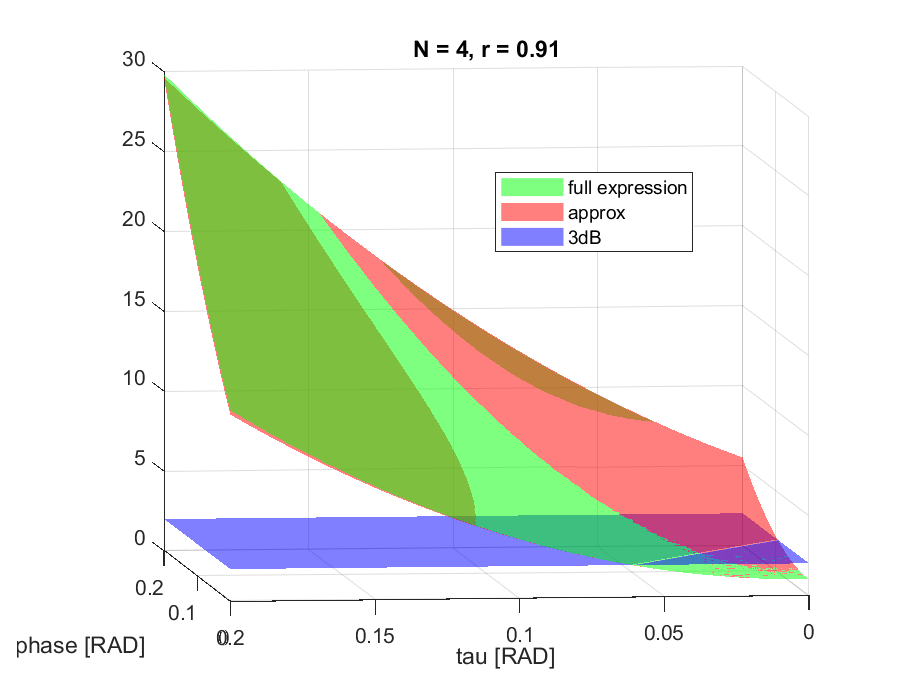
\includegraphics[width=0.9\linewidth]{./Media/spatial_IIR_MATLAB/beamwidth/BW_approx_validation.eps}
    \caption{Graphically comparing (\ref{eqn_arrayPerformance_beamwidth_fullEpxr}) and (\ref{eqn_arrayPerformance_beamwidth_approx}) for $N=4$ and $\rho=0.91$. The approximation seems to closely match the original expression.}
\end{figure}
Unlike the passive ULA case, it is evident from figure (\ref{fig_singleFreqFeedback_2ndTaylorNumericalValidation}) that the $4^{th}$ order terms are not needed for the evaluation of $\theta_{HPBW}$. In perfect phase alignment (i.e. $\Delta_{\tau}=0$), the u-space expression for the HPBW is $$u_{HPBW} =
\frac{
\left|1-\rho\right|
}{
\pi{d}
}
\lambda
\sqrt{\frac{
12
}{
\left(N-1\right)\left(\left(1+2r\right)N-4r+1\right)
}}.
$$
Comparing to the classic ULA beamwidth \cite{VanTrees2002DetectionIV}, thoroughly discussed in appendix \ref{appendix_theULABeamwidth}, we can express the improvement factor as
$$
\frac{
0.89\frac{\lambda}{ND}
}{
\theta_{HPBW,IIR}
}
=
\frac{0.89}{\left|1-\rho\right|}\sqrt{\frac{1+2r}{12}}
$$
\todo{TODO}
\textbf{Add graph of the improvement factor}
% \subsection{The pole-based design approach}
% In this approach, we look for setting the response "poles" which minimize the denominator, thus maximizing the overall response magnitude. To evaluate the beamwidth, we chose to allocate all of the system's poles in a single position such that 
% $
% 1-\vecnot{\beta}^{T}\vecnot{d}_{\theta}e^{-j\tau}
% =
% \left(e^{j\theta}-re^{j\theta_{s}}\right)^{N}
% $
% where $N$ is the number of array sensors and $r \in \left[0,1\right)$ enables us to avoid treatment of $\infty$-valued expressions. Next, we look for $\theta$ such that
% $
% \left|\frac{
% \frac
% {
% \vecnot{\alpha}^{T}\vecnot{d}_{\theta_{s}}
% }{
% \vecnot{\beta}^{T}\vecnot{d}_{\theta_{s}}
% }
% }{
% \frac
% {
% \vecnot{\alpha}^{T}\vecnot{d}_{\theta}
% }{
% \vecnot{\beta}^{T}\vecnot{d}_{\theta}
% }
% }\right|
% = \frac{1}{\sqrt{2}}
% $. Assuming that, like in classical IIR filter design theory, the numerator behaviour is significantly "slower" than the denominator's which results in $\vecnot{\alpha}^{T}\vecnot{d}_{\theta} 
% \approx
% \vecnot{\alpha}^{T}\vecnot{d}_{\theta_{s}}$ reults in
% \begin{align*}
%     \left|\frac{
%     \vecnot{\beta}^{T}\vecnot{d}_{\theta}
%     }{
%     \vecnot{\beta}^{T}\vecnot{d}_{\theta_{s}}
%     }\right|
%     &= \frac{1}{\sqrt{2}}
%     \\
%     \left|
%     \frac{
%     \left(e^{j\theta}-re^{j\theta}\right)^{N}
%     }{
%     \left(e^{j\theta}-re^{j\theta_{s}}\right)^{N}
%     }
%     \right|
%     &=
%     \left|
%     \frac{
%     \left(1-re^{j\left(\theta_{s}-\theta\right)}\right)
%     }{
%     \left(1-r\right)
%     }
%     \right|^{N}
%     \\
%     &=
%     \left|
%     \frac{
%     1+r^{2}-2r\cos{\left(\theta_{s}-\theta\right)}
%     }{
%     \left(1-r\right)^{2}
%     }
%     \right|^{\frac{N}{2}}
%     =
%     \left(\frac{1}{2}\right)^{\frac{1}{2}}
%     \\
%     \Rightarrow 
%     1+r^{2}-2r\cos{\left(\theta_{s}-\theta\right)}
%     &=
%     \left(1-r\right)^{2}2^{\frac{1}{N}}
%     \\
%     \cos{\left(\theta_{s}-\theta\right)}
%     &=
%     \frac{
%     1+r^{2}-\left(1-r\right)^{2}2^{\frac{1}{N}}
%     }{
%     2r
%     }
%     \\
%     \Rightarrow
%     \frac{\omega{D\left(cos(\theta_{g,s})-cos(\theta_{g,B})\right)}}{c}
%     &=
%     cos^{-1}
%     \left(
%     \frac{1+r^{2}-\left(1-r\right)^{2}2^{\frac{1}{N}}}{2r}
%     \right)
% \end{align*}.
% Therefore,
% \begin{equation}
%     \theta_{g,B} 
%     &= 
%     cos^{-1}
%     \left(
%     cos(\theta_{g,s})
%     -
%     \frac{c}{\omega{D}}
%     cos^{-1}
%     \left(
%     \frac{1+r^{2}-\left(1-r\right)^{2}2^{\frac{1}{N}}}{2r}
%     \right)
%     \right)
% \end{equation}
% Few observations can be derived from the $ \theta_{g,B} $:
% \begin{itemize}
%     \item $r\rightarrow{1}$ (i.e. setting the pole on the unit circle) causes $\theta_{g,B}\rightarrow\theta_{g,s}$ due to the $\infty$ valued response at $\theta_{g,s}$
%     \item The interval 
%     $
%     \left\{
%     \theta_{g,s}
%     \ \Bigg{|}\ 
%     cos(\theta_{g,s})
%     -
%     \frac{c}{\omega{D}}
%     cos^{-1}
%     \left(
%     \frac{1+r^{2}-\left(1-r\right)^{2}2^{\frac{1}{N}}}{2r}
%     \right)
%     <-1
%     \right\}
%     $, has no solution. In simulations, when evaluating such $\theta_{g,s}$ values, one can observe that the actual beampattern does not resemble the designed one due to the ULA geometric properties.
%     \item The number of sensors $N$ seems to have low impact on the beamwidth.
% \end{itemize}
\subsection*{Location of sidelobes and the rate of decrease}
Unlike the passive ULA case, it is clear from (\ref{eqn_arrPerformance_beamwidth_3dB}) that the positions of the feedback based beampattern sidelobes are affected both by the numerator and the denominator of $\Hr_{\dTheta}$. Considering the \coefSetName{} approach (i.e. single DOA enhancement), the denominator has only one single minima on the main lobe. Therefore, the sidelobes positions, same as the ULA case, are known \cite{VanTrees2002DetectionIV} to be 
\begin{equation}
    \label{eqn_CB_sidelobesLocations}
    \dTheta_{\coefSetName{},\text{sidelobes}} = \frac{\rBrace{2m+1}\pi}{N}\ \forall m\in\cBrace{1,2,\hdots}.
\end{equation}
Our initial interest is the first sidelobe (i.e. $m=1$), therefore we express the normalized beampattern at $\dTheta = \frac{3\pi}{N}$ (and setting $\dPhi=0$ for objective comparison). It can easily be verified that 
\begin{equation*}
    \Hr_{\frac{3\pi}{N}}
    =
    \frac{
    2\rBrace{1-r}^{2}
    }{
    \rBrace{N^{2}-2Nr}\rBrace{1-\cos{\rBrace{\frac{3\pi}{N}}}}+2r^{2}
    },
\end{equation*}
which for large $N$ values (as seen in Fig.~\ref{fig_firstSidelobeGain_CB}), can be well approximated by
\begin{equation*}
    \sqrt{\Hr_{\frac{3\pi}{N}}}
    \overset{N\gg1}{\approx}
    \frac{
    2\rBrace{1-r}
    }{
    3\pi
    }.
\end{equation*}
\begin{figure}[t!]
    \begin{center}
        \begin{overpic}[width=.75\linewidth, 
        %grid, 
        tics=10,trim=0 0 0 0]{./Media/spatial_IIR_MATLAB/arrayParameters/firstSidelobeGain_vs_N_various_r.eps}
            \put (6, 72){\footnotesize{$\Hr_{\frac{3\pi}{N}}{}$ - First sidelobe gain}}
            \put (20, 54) {\footnotesize{$r=0$ (i.e. no feedback)}}
            \put (20, 42) {\footnotesize{$r=0.3$}}
            \put (20, 33) {\footnotesize{$r=0.5$}}
            \put (20, 24) {\footnotesize{$r=0.7$}}
            \put (20, 14) {\footnotesize{$r=0.9$}}
            \put (-3, 50.5) {{$\frac{2\rBrace{1-0}}{3\pi}$}}
            \put (-3, 37.5) {{$\frac{2\rBrace{1-0.3}}{3\pi}$}}
            \put (-3, 28.5) {{$\frac{2\rBrace{1-0.5}}{3\pi}$}}
            \put (-3, 20) {{$\frac{2\rBrace{1-0.7}}{3\pi}$}}
            \put (-3, 12) {{$\frac{2\rBrace{1-0.9}}{3\pi}$}}
            \put (50, 2) {\footnotesize{$N$}}
        \end{overpic}
    \end{center}
    \caption{Plot of $\Hr_{\frac{3\pi}{N}}{}$ (i.e. the first sidelobe gain) vs. N for various $r$ values. The expected limit values (for large $N$) are presented as horizontal lines for each instance of $r$. Evidently, as expected, the gains tend to unite with the matching limits. $r=0$ is of special importance, being the reference for evaluation of the integrated feedback related improvement.}
    \label{fig_firstSidelobeGain_CB}
\end{figure}
It follows that, comparing to the known \cite{VanTrees2002DetectionIV} result of the passive ULA case (i.e. first sidelobe gain of $\frac{2}{3\pi}$), the first sidelobe gain improvement factor under the \coefSetName{} approach is
\begin{equation}
    \mu_{\text{first-sidelobe-gain,\coefSetName{}}} = \frac{1}{1-r}.
\end{equation}
Since the denominator magnitude, under the \coefSetName{} approach, is practically flat when not around the main lobe, the rate of sidelobes decay stays approximately the same as the numerators, which is similar to the known \cite{VanTrees2002DetectionIV} passive ULA sidelobe decay rate of $1/\rBrace{2m+1}$ (where $m$ is the sidelobe index).
\subsection*{Array directivity}
Another common measure for the array performance is the directivity \cite{VanTrees2002DetectionIV}, $\text{D}$. In the context of this work, considering the steer error scenario, it is defined as
\begin{equation*}
    \text{D}_{\coefSetName{}} = \frac{\Hr_{0}}{\frac{1}{2\pi}\int^{0}_{2\pi}\Hr_{\dTheta}\ d\dTheta},
\end{equation*}
measuring the ratio between the maximal array gain to the averaged gains in all directions. For uniformly weighted passive ULAs, assuming normalized beampattern, it is known \cite{VanTrees2002DetectionIV} that $D = N$.
\par Numerically sweeping various $\vBrace{N,r}$ sets, unveils that
\begin{equation}
    \text{D}_{\coefSetName{}} = \frac{r^{2}-\rBrace{N-1}r+N}{\rBrace{r-1}^{2}},
\end{equation}
matching the passive ULA result (i.e. $\evalat{D_{ULA}}{r=0}=N$), which leads to expressing the \coefSetName{} directivity improvement factor 
\begin{equation}
    \mu_{\text{D},\coefSetName{}}= \frac{r^{2}-\rBrace{N-1}r+N}{N\rBrace{r-1}^{2}}\overset{N\to\infty}{\to}\frac{1}{\rBrace{r-1}}.
\end{equation}
It is worth mentioning that for $\vBrace{r\to1,N\gg1}$ value sets, classic numerical approximations for the integral fail around $\dTheta\to0$ due to the the fact that both the numerator and the denominator tend to 0 (known to have a finite limit of 1 for $\dTheta=0$), forcing symbolic evaluation which was achieved using MATHEMATICA.
\section{Range Error Sensitivity}
\label{sec_sim}
% In this section, we first aim to validate the derivations of Sec.~\ref{sec_introduceFeedback}, while still considering the steer error scenario. Time domain simulations are presented in Fig.~\ref{fig_steerErrorTemporalSim}, showing perfect match between the simulations and the expected spatial response (\ref{eqn:GeneralFeedbackTransferFunction}).
% \begin{figure}[t!]
%   \centering
%   \subfloat[][]{\begin{overpic}[width=.45\linewidth, 
%         % grid, 
%         tics=10,trim=0 0 0 0]{./Media/h_thetaTau/steerError_r0.png}
%             \put (12, 72){\tiny{$\lBrace{h\rBrace{\dTheta}}, r=0$}}
%             \put (65, 65){\tiny{Expected pattern}}
%             \put (65, 61) {\tiny{Simulation results}}
%             \put (49, -1) {\tiny{$\dTheta\vBrace{RAD}$}}
%             \put (0, 40) {\tiny{dB}}
%         \end{overpic}\label{subfig_steerErrorTemporalSim_r0}}\quad
%   \subfloat[][]{\begin{overpic}[width=.45\linewidth, 
%         % grid, 
%         tics=10,trim=0 0 0 0]{./Media/h_thetaTau/steerError_r06.png}
%             \put (12, 72){\tiny{$\lBrace{h\rBrace{\dTheta}}, r=0.6$}}
%             \put (49, -1) {\tiny{$\dTheta$}}
%             \put (0, 40) {\tiny{dB}}
%         \end{overpic}\label{subfig_steerErrorTemporalSim_r06}}\\
%   \subfloat[][]{\begin{overpic}[width=.45\linewidth, 
%         % grid, 
%         tics=10,trim=0 0 0 0]{./Media/h_thetaTau/steerError_r08.png}
%             \put (12, 72){\tiny{$\lBrace{h\rBrace{\dTheta}}, r=0.8$}}
%             \put (49, -1) {\tiny{$\dTheta$}}
%             \put (0, 40) {\tiny{dB}}
%         \end{overpic}\label{subfig_steerErrorTemporalSim_r08}}\quad
%   \subfloat[][]{\begin{overpic}[width=.45\linewidth, 
%         % grid, 
%         tics=10,trim=0 0 0 0]{./Media/h_thetaTau/steerError_r095.png}
%             \put (12, 72){\tiny{$\lBrace{h\rBrace{\dTheta}}, r=0.95$}}
%             \put (49, -1) {\tiny{$\dTheta$}}
%             \put (0, 40) {\tiny{dB}}
%         \end{overpic}\label{subfig_steerErrorTemporalSim_r095}}
%   \caption{For simulating the system's spatial response, we considered the steer-error case only in acoustic environment, where the signal's frequency is $10_{kHz}$ and steered a feedback-based array of $3$ elements towards the end-fire direction. For each $r$ value, we generate multiple simulations of a far-field target in different angular positions, covering $\theta_{g}\in\vBrace{0,\pi}$ and for each $\theta_{g}$ we plot the final array output magnitude. Each simulation was $100$ iterations long, where one iteration is the time that takes for a signal to get to the target, reflect and re-impinge the array. In \ref{subfig_steerErrorTemporalSim_r0} we simulate the passive array ($r=0$) for reference. Introducing the feedback, \ref{subfig_steerErrorTemporalSim_r06},\ref{subfig_steerErrorTemporalSim_r08} and \ref{subfig_steerErrorTemporalSim_r095} are simulations of the same array with $r$ values of $0.6, 0.8$ and $0.95$ respectively. The reader may observe that the beampattern sharpens and the side-lobes are decayed as $r$ increases, as predicted in Sec.~\ref{sec_Performance}.}
%   \label{fig_steerErrorTemporalSim}
% \end{figure}
In this section we investigate $\Hr_{\dTheta,\dPhi,r}\rBrace{\omega}$ of \eqref{eq_generalH} for the general case, where the range misalignment phase term $\dPhi$ is possibly non zero. In Fig.~\ref{fig_hDUDTContour}, we plot $\abs{\Hr_{\dTheta,\dPhi,r}\rBrace{\omega}}$ in logarithmic scale, with respect to both steer and range misalignments. 
We first note that the sensitivity to range errors is  $2\pi$-periodic in $\dPhi$, as also evident from \eqref{eq_generalH}, and demonstrated in Fig.~\ref{fig_hDUDTContour_mutliPeak}.
One can also observe that as $r$ tends to one, this significantly sharpens the spatial selectivity of the system. Unfortunately, the response is very sensitive to range errors, as the main beam is supported on a small interval along the $\dPhi/\pi$ axis.
As we defined
\[
\phi\triangleq\omega\tau_{pd}=\frac{2\pi R_{rt}}{\lambda}
\]
where $R_{rt}$ is the round-trip distance between the array and the target of interest, we can express range errors as
\[
\Delta R_{rt}=\frac{\dPhi \lambda}{2\pi}. 
\]
The range related sensitivity is also emphasized in Fig.~\ref{fig_rangError}, demonstrating that even minor range errors significantly distort the beampattern.
\par At first glance, this sensitivity to range errors renders the system being too sensitive for any practical use.
\begin{figure}[t!]
    \begin{center}
        \begin{overpic}[width=.95\linewidth, 
        % grid, 
        tics=10,
        % trim={<left> <lower> <right> <upper>}
        trim={0cm 0cm 1.5cm 0cm}
        ]{./Media/spatialIIR_amb_N3_all_r.eps}
            \put (91, 74) {\footnotesize{dB}}
            %\put (43, 57.5) {$\frac{\dPhi}{\pi}$}
            %\put (43, 22) {$\frac{\dPhi}{\pi}$}
            %\put (-2, 57.5) {$\frac{\dPhi}{\pi}$}
            \put (-2, 22) {$\frac{\dPhi}{\pi}$}
            \put (5, 74) {\footnotesize{$r=0.4$}}
            \put (51, 74) {\footnotesize{$r=0.6$}}
            \put (5, 38) {\footnotesize{$r=0.7$}}
            \put (51, 38) {\footnotesize{$r=0.8$}}
            \put (19, 3) {\footnotesize{$\dTheta/\pi$}}
            %\put (65, 3) {\footnotesize{$\dTheta/\pi$}}
            %\put (19, 43) {\footnotesize{$\dTheta/\pi$}}
            %\put (65, 43) {\footnotesize{$\dTheta/\pi$}}
            % \put (21, 44) {\footnotesize{(a)}}
            % \put (21, -1) {\footnotesize{(c)}}
            % \put (67, 44) {\footnotesize{(b)}}
            % \put (67, -1) {\footnotesize{(d)}}

        \end{overpic}
    \end{center}
    \caption{Evaluation of $10\log_{10}\abs{\Hr_{\dTheta,\dPhi,r}}^2$, considering both steer ($\dTheta$) and range related ($\dPhi$) errors. Centered in each plot, is the 3dB main lobe (white color fill), exemplifying that as the gain mismatch $r$ is set closer to one, we observe an increase of the spatial selectivity (regarding  both $\dTheta$ and $\dPhi$).}
  \label{fig_hDUDTContour}
\end{figure}
\begin{figure}[t!]
    \begin{center}
        \begin{overpic}[width=0.6\linewidth, 
        % grid, 
        tics=10,
        % trim={<left> <lower> <right> <upper>}
        trim={0 0 0 0}
        ]{./Media/spatialIIR_amb_N3r04_multiPeak.eps}
            \put (83, 71) {\tiny{dB}}
            \put (42, -0.5) {\scriptsize{$\dTheta/\pi$}}
            \put (0, 37) {$\frac{\dPhi}{\pi}$}
        \end{overpic}
    \end{center}
    \caption{Evaluation of $10\log_{10}\abs{\Hr_{\dTheta,\dPhi,r=0.4}}^2$ for $-3\pi\leq\dPhi\leq 3\pi$. The response is $2\pi$ periodic.}
  \label{fig_hDUDTContour_mutliPeak}
\end{figure}
\begin{figure}[t!]
    \begin{center}
        \begin{overpic}[width=0.7\linewidth, 
        % grid, 
        tics=10,
        % trim={<left> <lower> <right> <upper>}
        trim={0 0 0 0}
        ]{./Media/rangeError_r06.eps}
            \put (-1, 74) {\footnotesize{$10\log_{10}\abs{\Hr_{\dTheta,\dPhi,r}}^2$}}
            \put (46, -1) {\footnotesize{$\dTheta/\pi$}}
            \put (0, 37) {\footnotesize{dB}}
            \put (92, 40) {\footnotesize{$\Delta R_{rt}=0.1\lambda$}}
            \put (92, 50) {\footnotesize{$\Delta R_{rt}=0.3\lambda$}}
            \put (92, 30) {\footnotesize{$\Delta R_{rt}=0$}}
        \end{overpic}
    \end{center}
    \caption{Evaluation of the array response for several values of range error $\Delta R_{rt}$ (where $r=0.4$). Even minor range errors significantly distort the beampattern.}
  \label{fig_rangError}
\end{figure}
This leads us to seek robust implementations, as demonstrated in Sec.~\ref{sec_app}. 

\section{Mitigating Range Error Sensitivity}
\label{sec_app}
As demonstrated in the previous section, the beampattern \eqref{eq_generalH} is very sensitive to range errors.
We now propose an architecture which obtains the desired beampattern $\Hr_{\dTheta,\dPhi\to0,r}$ even when in practice, the true range to the target is unknown (i.e. $\Delta R_{rt}$ is large). Moreover, we intend to show that the suggested architecture operates at moderately low signal to noise ratio (SNR).

\subsection*{Motivation}
Bearing in mind that the system's phase alignment sensitivity resides in \eqref{eq_generalH} via the  term $\exp\Brack{j\dPhi}=\exp\Brack{j\omega\Delta\tau_{pd}}$, and that the round-trip delay (i.e. $\tau_{pd}$) cannot be controlled, one may suggest to use lower frequencies. Unfortunately, transmission of such low frequencies is physically unfeasible. 
\par Another approach is to simultaneously use several frequencies in order to resolve the range error sensitivity. In the following, we show a possible algorithm which achieves this goal by transmitting with two frequencies $\omega_1$ and $\omega_2$.

\subsection*{Suggested processing scheme}
\begin{figure}[t!]
    \begin{center}
        \begin{overpic}[width=0.95\linewidth, 
        % grid, 
        tics=10,trim={0 0 0 0}]{./Media/SpatialIIR_APP.png}
            \put (12.5, 64){$\text{FB}_{\vAlpha_{1},\vBeta_{1}}$}
            \put (61, 64){$\text{FB}_{\vAlpha_{2},\vBeta_{2}}$}
            \put (4.5, 59){$y_{1}\rBrace{t}$}
            \put (54, 59){$y_{2}\rBrace{t}$}
            \put (12.9, 41.5){$\text{BPF}_{\omega_{1}}$}
            \put (61.65, 41.5){$\text{BPF}_{\omega_{2}}$}
            \put (6, 51.5){+}
            \put (55, 51.5){+}
            \put (16, 51.5){\footnotesize{$n_{1}\rBrace{t}$}}
            \put (64.75, 51.5){\footnotesize{$n_{2}\rBrace{t}$}}
            \put (24.5, 59){\footnotesize{$\text{Tx}_{1}\rBrace{t}$}}
            \put (73.5, 59){\footnotesize{$\text{Tx}_{2}\rBrace{t}$}}
            \put (36.25, 64){\scriptsize{$x_{1}\rBrace{t}$}}
            \put (43, 64){\scriptsize{$x_{2}\rBrace{t}$}}
            \put (18.25, 13){\footnotesize{Harmonic mean}}
            \put (32, 2){$y\rBrace{t}$}
            \put (54.75, 24){$\Sigma$}
            \put (21.75, 25){\footnotesize{$\mathcal{F}_{\omega_{1}}$}}
            \put (30.75, 25){\footnotesize{$\mathcal{F}_{\omega_{2}}$}}
        \end{overpic}
    \end{center}
    \caption{Dual-frequency beamformer, consisting of two independent FB blocks and nerrwoband bandpass filters. The blocks marked by $\mathcal{F}_{\omega_{i}}$ compute the Fourier coefficients in $\omega_{i}$ and their outputs feed the harmonic mean calculator which generates the DF beamformer's output.}
    \label{fig_app}
\end{figure}
In Fig.~\ref{fig_app}, we exemplify the use of two independently configured instances of the feedback beamformer (of Fig.~\ref{fig:Proposed_spatialIIR_ARCH}), where each instance is designed to treat only a specific frequency. 
\par For this, two independent FB blocks and 4 nerrow-band band-pass-filters ($\text{BPF}_{\omega_{i}}$ filters a nerrow band slice around $\omega_{i}$) are used to generate both the transmitted feedback signal ($\text{Tx}_{i}$) and the beamformers' outputs $y_{i}$. 
\par Also, $x_{i}(t) = e^{j\omega_{i}t}, \omega_{i} = 2\pi{f_{i}}$ with $i=1,2$ are two independent, narrow band, stimuli signals and $n_{i}$ are additive noise instances. 
\par Note that we do not increase the number of array elements, but merely double the beamformer processing part. 
\par For each single frequency FB block \eqref{eqn:GeneralFeedbackTransferFunction} the output is
\[
y_{i}(t)=H_{\vAlpha_{i},\vBeta_{i}}\rBrace{\omega_{i}}\exp{\rBrace{j\omega_{i}t}}\ \ {i\in\cBrace{1,2}},
\]
where $\vAlpha_{i},\vBeta_{i}$ are the coefficients of the $i$'th beamformer. 
\par We define $H_{\text{DF}}$ to be the \textit{dual frequency} beamformer, which is computed as the harmonic mean of $H_{\vAlpha_{i},\vBeta_{i}}(\omega_i)$ 
\begin{equation*}
    H_{\text{DF}} = \rBrace{H^{-1}_{\vAlpha_{1},\vBeta_{1}}\rBrace{\omega_{1}}+H^{-1}_{\vAlpha_{2},\vBeta_{2}}\rBrace{\omega_{2}}}^{-1}.
\end{equation*}
In practice, $H_{\text{DF}}$ can be estimated by evaluating $y_1(t)$ and $y_2(t)$ in the frequency domain, as also illustrated in Fig.~\ref{fig_app}.

By straight forward derivations, one may deduce that $\lBrace{H_{\text{DF}}}^{-1}$ is
% \begin{equation*}
%     \resizebox{1\linewidth}{!}{
%         \begin{split}
%             \lBrace{H_{\text{DF}}} =
%             \lBrace{
%             \frac
%             {
%             \vBetaT_{1}\vd_{1}\vBetaT_{2}\vd_{2}
%             }{
%             \vBetaT_{2}\vd_{2}\exp{\rBrace{-j\rBrace{\phi_{1}-\phi_{2}}}}+\vBetaT_{1}\vd_{1}
%             -\rBrace{\vBetaT_{1}\vd_{1}\vAlphaT_{2}\vd_{2}+\vBetaT_{2}\vd_{2}\vAlphaT_{1}\vd_{1}}\exp{\rBrace{-j\phi_{2}}}
%             }
%             }.
%         \end{split}
%     }
% \end{equation*}
\begin{equation*}
    \resizebox{1\linewidth}{!}{
        \begin{split}
            \lBrace{
            \frac
            {
            \vBetaT_{2}\vd_{2}\exp{\rBrace{j\rBrace{\phi_{1}-\phi_{2}}}}+\vBetaT_{1}\vd_{1}
            }{
            \vBetaT_{1}\vd_{1}\vBetaT_{2}\vd_{2}
            }
            -
            \frac
            {
            \rBrace{\vBetaT_{1}\vd_{1}\vAlphaT_{2}\vd_{2}+\vBetaT_{2}\vd_{2}\vAlphaT_{1}\vd_{1}}\exp{\rBrace{-j\phi_{2}}}
            }{
            \vBetaT_{1}\vd_{1}\vBetaT_{2}\vd_{2}
            }
            }.
        \end{split}
    }
\end{equation*}
Note that in the special case of choosing $\vAlpha_{1}~=~\vBeta_{1},\ \vAlpha_{2}~=~-~\vBeta_2{}$, the resultant beampattern simplifies to
\begin{equation}
    \label{eqn_twoFreqApproach_h}
    \abs{H_{\text{DF}}} = \lBrace{\frac{\vBetaT_{1}\vd_{1}}{1+\frac{\vBetaT_{1}\vd_{1}}{\vBetaT_{2}\vd_{2}}\exp{\rBrace{-j\rBrace{\phi_{1}-\phi_{2}}}}}}.
\end{equation}
\par In the general case, the gain of each element is frequency dependant, such that the steering vector $\vd$ of \eqref{eq:d}
may be expressed as 
\begin{equation*}
    \vd_{\theta_g}[n] = g_{n,\theta_{g}}(\omega)\exp{\rBrace{-j\omega\tau_{n,\theta_g}}},\;n=0,\ldots,N-1.
\end{equation*}
To simplify the exposition, we assume common gain across the array (i.e. $g_{\theta_{g}}(\omega)$ is not a function of the element index $n$) and suppress the DOA ($\theta_g$) dependency (which is the same at both frequencies) such that one may express the $i$'th frequency steering vector as
\begin{equation}\label{eq:new_d}
\vd_{i}^T=g(\omega_i)\sBrack{\exp{\rBrace{-j\omega_i\tau_{0}}},...,\exp{\rBrace{-j\omega_i\tau_{N-1}}}}.
\end{equation}
\par Note that the element-wise delay $\tau_n$ is arbitrary, hence we no longer restrict the discussion to linear arrays or any specific array manifold. Also, as $\tau_n$ represents the inter-element delay, we use $\tau_0=0$ (i.e. treating sensor $0$ as the reference sensor).
\par We further simplify the second beamformer's weights to 
\begin{equation}\label{eq_simpleBeta}
    \vAlpha_{2}=-\vBeta_{2}=\vBrace{\hat{g}^{-1}(\omega_2),0,\hdots,0}.
\end{equation}
Plugging \eqref{eq_simpleBeta} into \eqref{eqn_twoFreqApproach_h} gives rise to 
\begin{equation}
    H_{\text{DF}} = \lBrace{\frac{\vBetaT_{1}\vd_{1}}{1+
    \rBrace{\vBetaT_{1}\vd_{1}/r_{2}}\exp\rBrace{-j\rBrace{\phi_{1}-\phi_{2}}}
    }},
    \label{eq_H_DF_general}
\end{equation}
where $r_i=g(\omega_i)/\hat{g}(\omega_i)$ is the gain mismatch at $\omega_i$. 
\par Notice that  $H_{\text{DF}}$ is similar to the single frequency (SF) beampattern \eqref{eqn:GeneralFeedbackTransferFunction}, where the range related phase $\phi$ is replaced by $\phi_{1}-\phi_{2}=(\omega_1-\omega_2)\tau_{pd}$. Hence, by using sufficiently close frequencies, one may significantly mitigate the range mismatch distortion of the beampattern.
\par For example, consider a radio frequency carrier of $10\text{GHz}$ and typical range error of $\Delta{}R_{rt}=10_m$, which is $333\frac{1}{3}\lambda$ (assuming light speed of $c=3\cdot 10^{8}_{m/s}$). The single frequency beampattern distortion, being periodic in $\lambda$, will closely resembles the $0.3\lambda$ error plot presented in Fig.~\ref{fig_rangError}. 
\par Assume that we aim at maximal phase error of $\Delta \phi=0.01\pi_{rad}$. Hence, when using the \textit{dual frequency} architecture, the dictated frequency relation is
\begin{equation}\label{eq_DF_phErr}
\abs{(\omega_1-\omega_2)\frac{\Delta{}R_{rt}}{c}}<0.01\pi.
\end{equation}
or equivalently, for maximal range error of $10_m$, frequency separation of
\[
\abs{f_1-f_2}<0.005 c/\Delta{}R_{rt}=150_{KHz}
\]
is required. 

\subsection*{Dual frequency $\coefSetName$ simulation}
We now simulate \eqref{eq_H_DF_general} for the $\coefSetName$ approach assuming ULA. Using coefficients $\vBeta_{1}$ which will coherently sum the wave-front, while minimizing the magnitude of the denominator, we use
\begin{equation*}
    \vBeta_{1}=-\hat{\vd}^{\ast}\exp\rBrace{j\rBrace{\hat{\phi}_{1}-\hat{\phi}_{2}}}/\norm{\hat{\vd}}^2
\end{equation*}
where $\hat{\vd}$ is the estimated steering vector, as in \eqref{eq:d_hat}. With this choice, and similarly to \eqref{eq:SF_CB}, \eqref{eq_H_DF_general} becomes
\begin{equation}
    \label{eqn_H_DF_CB}
    \resizebox{.89\linewidth}{!}{
        \begin{split}
            H_{\text{DF,CB}} =
            \lBrace{\frac{r_{1}\D{\dTheta/2}{N}}{1-
            \kappa\D{\dTheta/2}{N}\exp\rBrace{-j\rBrace{\dPhi_{2}-\dPhi_{1}+(N-1)\dTheta/2}}}
            },
        \end{split}
    }
\end{equation}
where $\kappa\triangleq{}r_{1}/r_{2}$ is the gain mismatch ratio.
\par Note that for close frequencies such that $r_{1}\sim{}r_{2}$, $\kappa$ tends towards unity, thus significantly mitigating the gain mismatch effect even when both feedback beamformers are mismatched.
\par In Fig.~\ref{fig_dualfreq_rangeErrorHighSnr}, we simulate the beampattern (normalized to $0$dB peak gain) for the single and \textit{dual frequency} architectures, where frequency separation was configured to obtain range errors as in \eqref{eq_DF_phErr} (i.e. $f_1=10_{GHz},\;f_2=f_1+150_{KHz}$ to mitigate range errors up till $\Delta{}R_{rt}=10_m=333\frac{1}{3}\lambda$). 
\par We also plot (in blue circles) the perfectly aligned pattern, which is obtained when there are no range errors. 
\par As can be seen, the resultant beampattern of the \textit{dual frequency} beamformer practically achieves the ideal, range-error free case. 

In Fig.~\ref{fig_dualfreq_perfectAlignLowSnr}
we repeat the case of fractional range error of $\Delta{}R_{rt}=0.3\lambda$, while adding white Gaussian noise to the output of each feedback beamformer. Evidently, the dual-frequency beamformer (green diamonds) achieves close-to-ideal beampattern (blue circles), while the single-frequency beamformer (red squares) suffers severe distortions.
\begin{figure}[t!]
    \begin{center}
        \begin{overpic}[width=.7\linewidth, 
        % grid, 
        tics=10,trim=0 0 0 0]{./Media/fig_dualfreq_rangeErrorHighSnr.eps}
            \put (48, 43){\scriptsize{Ideal}}
            \put (48, 37.5){\scriptsize{SF}}
            \put (48, 32){\scriptsize{DF}}
            \put (2, 37.5){\footnotesize{dB}}
            \put (47,0){\footnotesize{$\dTheta/\pi$}}
            \put (92,58){\footnotesize{$\Delta{}R_{rt}=0.3\lambda$}}
        \end{overpic}
    \end{center}
    \caption{Simulating 3 element ULA with $r_1=0.6^{2},\; r_2=0.6$ (hence $\kappa=0.6$) for infinite SNR. The (fractional) range error is $\Delta{}R_{rt}=0.3\lambda$.
    The ideal response is obtained for $\Delta{}R_{rt}=0$ (blue dots), with the single frequency (SF) beamformer (red squares) and the  dual-frequency (DF) solution (green diamonds). 
    }
    \label{fig_dualfreq_rangeErrorHighSnr}
\end{figure}
\begin{figure}[t!]
    \begin{center}
        \begin{overpic}[width=0.9\linewidth, 
        % grid, 
        tics=10,
        % trim={<left> <lower> <right> <upper>}
        trim={1.75cm 0 1.75cm 0}
        ]{./Media/fig_dualfreq_rangeErrorLowSnr.eps}
            \put (42.25, 17.5){\scriptsize{Ideal}}
            \put (42.25, 14.5){\scriptsize{SF}}
            \put (42.25, 11.5){\scriptsize{DF}}
            \put (-1, 26.5){\footnotesize{dB}}
            \put (22, 0){\footnotesize{$\dTheta/\pi$}}
            \put (19,17){\scriptsize{$\text{SNR}=6_{dB}$}}
            \put (71.5,17){\scriptsize{$\text{SNR}=0_{dB}$}}
        \end{overpic}
    \end{center}
    \caption{Directional response of the 3 element ULA, as in Fig.~\ref{fig_dualfreq_rangeErrorHighSnr}, simulated for the noisy scenario. The additive noises $n_1(t)$ and $n_2(t)$ (see Fig.~\ref{fig_app}), are set to obtain SNR of $6_{dB}$ (left plot) and $0_{dB}$ (right plot).}
    \label{fig_dualfreq_perfectAlignLowSnr}
\end{figure}
% needed in second column of first page if using \IEEEpubid
%\IEEEpubidadjcol
%A possible evaluation for the contribution of the presented feedback mechanism is to measure the additional information in the system.
To this end, the FIM, denoted by $J$, will now be calculated with respect to the DOA parameter $\thetaD$ and the range related parameter $\phi$. 
As the feedback-based transfer function (\ref{eqn:GeneralFeedbackTransferFunction}) is expressed in frequency domain, we rely on \cite{zeira1990frequency} to express the frequency domain FIM as well. 
\par A single FIM element, may be expressed as
\begin{equation}\label{eq_FIM_kl_full}
    \resizebox{.9\linewidth}{!}{
        \begin{split}
            J_{\vBrace{k,l}}\rBrace{\vEta} 
            =&
            \Re\cBrace{
            \frac{1}{2\pi}
            \int_{-\omega_{s}/2}^{\omega_{s}/2}
            {
            \frac{1}{\Phi\rBrace{\omega}}
            \mathfrak{F}^{*}\left\{
            \frac{\partial z(t)}{\partial\eta_{k}}
            \right\}
            \mathfrak{F}\left\{
            \frac{\partial z(t)}{\partial\eta_{l}}
            \right\}
            d\omega
            }}
            \\ &+
            \frac{T}{4\pi}
            \int_{-\omega_{s}/2}^{\omega_{s}/2}
            \frac{1}{\Phi^{2}\rBrace{\omega}}
            \frac{\partial\Phi\rBrace{\omega}}{\partial\eta_{k}}
            \frac{\partial\Phi\rBrace{\omega}}{\partial\eta_{l}}
            d\omega
        \end{split}
    }
\end{equation}
where $ \vEta = [\thetaD,\phi]^{T} $ is the parameters vector, $\Re$ stands for the real-part extraction operator, $k,l \in\cBrace{1,2}$, $\Phi\rBrace{\omega}$ is the noise spectrum, $\mathfrak{F}$ is the Fourier transform operator, $T$ is the measurement observation interval and $\omega_{s}$ is the signal bandwidth. 
For simplicity, $\text{n}\rBrace{t}$ is assumed to be a white Gaussian with some constant power spectral density $\Phi(\omega)=\sigma^2$ and independent of the estimated parameters $\eta$, hence the second term vanishes. 
Assuming continuously differentiable functions, where order alteration of the Fourier transform and the differentiation operations is allowed, \eqref{eq_FIM_kl_full} simplifies to
\begin{equation}
    \label{eq_beamPatternFreqDomain_FIM}
    % \resizebox{1\linewidth}{!}{
        \begin{split}
            J_{\vBrace{k,l}}\rBrace{\vEta} = 
            \Re\cBrace{
            \frac{1}{2\pi\sigma^2}
            \int_{-\omega_{s}/2}^{\omega_{s}/2}
            {
            \rBrace{\frac{\partial{}\F{z}\rBrace{\omega}}{\partial\eta_{k}}}^{\ast}
            \frac{\partial{}\F{z}\rBrace{\omega}}{\partial\eta_{l}}
            d\omega
            }}
        \end{split}.
    % }
\end{equation}
As mentioned before, $g$ is independent of the estimated parameters, therefore
\begin{equation}\label{eq_vdDiff}
\frac{\partial\vd}{\partial\thetaD}=A\omegaB\vd
\end{equation}
where $A\omegaB$ is an $N\times{}N$ diagonal matrix and each of its diagonal elements may expressed as 
\[
A_{\vBrace{i,i}}\omegaB=-j\omega\frac{\partial \tau_{i}}{\partial{\thetaD}}\ \  \forall{i\in\cBrace{0\hdots{}N-1}}.
\]
To further simplify the analysis, without loss of generality, we use (in this section only) $g=1$.
In App.~\ref{apdx_clacFim} we compute the FIM terms, concluding that
\begin{equation}
    \label{eqn_FIMelements}
    \resizebox{.91\linewidth}{!}{
        \begin{split}
            &J_{\theta\theta}
            =
            \frac{1}{2\pi\sigma^{2}}\int_{-\omega_{s}/2}^{\omega_{s}/2}{\frac{
            \lBrace{\vBetaT{}A\omegaB\vd-\vBetaT{}B\omegaB\vAlpha\ePhi{-}}^{2}
            }{
            \lBrace{\rBrace{1-\aTd\ePhi{-}}^{2}}^{2}
            }\lBrace{\F{s}\rBrace{\omega}}^{2}d\omega}
            \\
            &J_{\phi\phi}
            =
            \frac{1}{2\pi\sigma^{2}}\int_{-\omega_{s}/2}^{\omega_{s}/2}{\frac{
            \lBrace{\bTd}^{2}
            }{
            \lBrace{\rBrace{1-\aTd\ePhi{-}}^{2}}^{2}
            }\lBrace{\F{s}\rBrace{\omega}}^{2}d\omega}
        \end{split}
    }
\end{equation}
where $B\omegaB\triangleq\vd\vdT{}A\omegaB-A\omegaB\vd\vdT$.
Moreover, using some mild assumptions and setting
\begin{equation}\label{eq_alphaBetaPropSteer}
    \vAlpha,\vBeta\propto\vd^{\ast},
\end{equation}
we show that the cross terms of the FIM are nullified, i.e. $J_{\theta\phi} = J_{\phi\theta}^{*}=0$.
\par 
Choosing the weights as in \eqref{eq_alphaBetaPropSteer} may be interpreted as a generalization of the DS beamformer, formerly referenced as the conventional beamformer (CB) \cite{van2004optimum}, which coherently integrate the impinging signal along the array elements.
The same choice of weights also minimizes the $\lBrace{1-\aTd\ePhi{-}}$ term, significantly increasing the available information, as predicted by the FIM.
It is worth mentioning that \eqref{eq_vdDiff} is relevant even for arbitrary (non-omni-directional) sensors when smooth and slowly changing radiation patterns are assumed.
In practice, though, there will be unavoidable errors, and perfect knowledge of the steering vector $\vd$ is not always available.
In Sec.~\ref{sec_Performance}, we quantify the effect of such estimation errors and discuss its influence on the array performance. 
%Many approaches may be considered while setting $\vecnot{\alpha},\vecnot{\beta}$ in order to achieve optimal utilization of the spatial IIR structure in (\ref{eqn:GeneralFeedbackTransferFunction}), all sharing the same purpose of minimizing the IIR component (i.e. the denominator) for specific spatially selected signals.
One naturally considered approach is the \textbf{dual-conventional-beamformer} (DCBF). In this approach, to achieve minimization of the IIR component,$ \vecnot{\beta}^{T}\vecnot{d}_{\theta_{s}}e^{-j\omega\tau_{s}} = 1 $ (where $\tau_{s}$ is determined by the target's location), in order to achieve the desired high spatial selectivity. Considering the array phase and gain mismatch, we present $\rho = re^{\Phi}$, which will function as the \textbf{array-mismatch-factor}. Combined with the \textbf{conventional beamformer} (\cite{VanTrees2002DetectionIV}) we set $ \vecnot{\alpha} = \vecnot{\beta} = \frac{\rho}{N}\vecnot{d^{*}_{s}e^{-j\tau_{s}}} $). Comparing the perfectly-aligned scenario $\left(\theta = \theta_{s}, \tau = \tau_{s}\right)$ with the general scenario, enables calculation of the half-power-beamwidth (\textbf{HPBW}) by setting $\left|\frac{H_{\theta_{s}\tau_{s}}\left(\omega{}\right)}{H_{\theta,\tau}\left(\omega{}\right)}\right|^{2} = 2$, which translates to 
\begin{align}
\label{eqn_arrPerformance_beamwidth_3dB}
\Hr{\theta}{\tau}{}
\triangleq
\fbBpRatio
=
2\ .
\end{align}
Defining $\D{N}{x} = \frac{\sin{Nx}}{\sin{x}}$ , and performing some algebraic simplification, one gets
\ifdefined\showDev
    \\
    \fbox{
    \begin{minipage}{.95\linewidth}
    \textbf{development specifics}
    $$
    \Hr{\theta}{\tau}{}
    =
    \left|
    \frac{
    \vecnot{\alpha}^{T}\vecnot{d}_{\theta_{s}}
    }{
    \vecnot{\alpha}^{T}\vecnot{d}_{\theta}
    }
    \frac{
    1-\vecnot{\beta}^{T}\vecnot{d}_{\theta}e^{-j\tau}
    }{
    1-\vecnot{\beta}^{T}\vecnot{d}_{\theta_{s}}e^{-j\tau_{s}}
    }
    \right|
    =
    \left|
    \frac{
    1
    }{
    \frac{1}{N}\vecnot{d}^{H}_{\theta_{s}}\vecnot{d}_{\theta}
    }
    \frac{
    1-\frac{\rho}{N}\vecnot{d}^{H}_{\theta_{s}}\vecnot{d}_{\theta}e^{j\Delta_{\tau}}
    }{
    1-\rho
    }
    \right|
    $$
    .Using the geometric progression sum of the steering vectors product,
    $$
    \vecnot{d}^{H}_{\theta_{s}}\vecnot{d}_{\theta} = \Sigma_{n=0}^{N-1}e^{j\left(\theta-\theta_{s}\right)}
    $$
    and defining $\Delta_{\theta} \triangleq \theta-\theta_{s}$ one gets
    $$
    \vecnot{d}^{H}_{\theta_{s}}\vecnot{d}_{\theta} = e^{j\frac{N-1}{2}\Delta_{\theta}}\D{N}{\dTheta}
    $$.
    Integrated into the last expression, it yields\\
    \resizebox{.95\linewidth}{!}{
    \begin{minipage}{\linewidth}
    \begin{align*}
    \left|
    \frac{
    1
    }{
    1-\rho
    }
    \frac{
    N-\rho\vecnot{d}^{H}_{\theta_{s}}\vecnot{d}_{\theta}e^{j\Delta_{\tau}}
    }{
    \vecnot{d}^{H}_{\theta_{s}}\vecnot{d}_{\theta}
    }
    \right|^{2}
    &=
    \left|
    \frac{
    1
    }{
    1-\rho
    }
    \left(
    N\Dp{N}{\dTheta/2}{-1}
    e^{-j\frac{N-1}{2}\Delta_{\theta}}
    - 
    \rho{}e^{j\Delta_{\tau}}
    \right)
    \right|^{2}
    \\&=
    \left|
    \frac{
    1
    }{
    1-\rho
    }
    \left(
    N\Dp{N}{\dTheta/2}{-1}
    - 
    \rho{}e^{j\left(\Delta_{\tau}+\frac{N-1}{2}\Delta_{\theta}\right)}
    \right)
    \right|^{2}
    \\
    &=
    \frac{1}{\left|1-\rho\right|^{2}}
    \left(
    N^{2}\Dp{N}{\dTheta/2}{-2}
    -2rN\Dp{N}{\dTheta/2}{-1}\cos{\left(\Phi+\Delta_{\tau}+\frac{N-1}{2}\Delta_{\theta}\right)}
    +r^{2}
    \right)
    \end{align*}
    \end{minipage}}
    \\
    where $ \Delta_{\tau} \triangleq \tau-\tau_{s}$
    \end{minipage}
    }
\else
\fi
\resizebox{.97\linewidth}{!}{
  \begin{minipage}{\linewidth}
      \begin{align}
        \nonumber
        \label{eqn_arrayPerformance_beamwidth_fullEpxr}
        \Hr{\theta}{\tau}{2}
        =
        \frac{1}{\left|1-\rho\right|^{2}}
        \Bigg(
        & 
        N^{2}\Dp{N}{\dTheta/2}{-2} 
        \\ \nonumber &
        - 2rN\Dp{N}{\dTheta/2}{-1}\cos{\left(\Phi+\Delta_{\tau} + \frac{N-1}{2}\Delta_{\theta}\right)}
        \\ & 
        + r^{2}\Bigg),
    \end{align}
  \end{minipage}
}
where $ \Delta_{\tau} \triangleq \tau-\tau_{s} $ and $ \Delta_{\theta} \triangleq \theta-\theta_{s}$.
which can be easily verified to tend to $ 1 $ when $ \Delta_{\tau},\Delta_{\theta} \rightarrow 0$. 
Following \cite{VanTrees2002DetectionIV}'s steps (discussed in section \ref{section_arrayPerformance_classicULA}), we start by investigating the first order taylor expansion,$$ \evalat{f\left(x,y\right)}{x\to{}a,y\to{}b} \approx f(a,b) + \evalat{\frac{\partial{f}}{\partial{x}}}{\left(x=a,x=b\right)}\left(x-a\right) + \frac{\partial{f}}{\partial{x}}\left(a,b\right) $$,of the expression.
Using L'Hôpital's rule to evaluate the derivatives, results in 
\resizebox{.97\linewidth}{!}{
  \begin{minipage}{\linewidth}
    \begin{align*}
        \Hr{\theta}{\tau}{2}
        \propto &
        1 
        \\ &
        - \left(r\left(N-1\right)\sin{\Delta_{\tau}}\right)\Delta_{\theta}
        \\ &
        -\left(2Nr\mathcal{D}^{-1}\left(N,\sfrac{\Delta}{2}\right)\sin{\left(\frac{N-1}{2}\frac{\Delta_{\theta}}{2}\right)}\right)\Delta_{\tau}.
    \end{align*}
  \end{minipage}
}
Observing that setting $\Delta{\tau},\Delta{\theta} = 0$ zeros the first order coefficients, leads us to express the second order terms, resulting in 
\resizebox{.97\linewidth}{!}{
  \begin{minipage}{\linewidth}
    \begin{align}
        \label{eqn_arrayPerformance_beamwidth_approx}
        \nonumber
        \Hr{\theta}{\tau}{2} 
        \approx 
        1
        +
        \frac{1}{\left|1-\rho\right|^{2}}
        \Bigg(&
        \frac{1}{12}\left(N-1\right)\left(\left(1+2r\right)N-4r+1\right)\Delta^{2}_{\theta}
        \\& \nonumber
        + r\Delta^{2}_{\tau}
        \\&
        + r\left(N-1\right)\Delta_{\theta}\Delta_{\tau}
        \Bigg).
    \end{align}
  \end{minipage}
}
\begin{figure}
    \todo{Refine graph (units , labels, title)}
    \label{fig_singleFreqFeedback_2ndTaylorNumericalValidation}
    \centering
    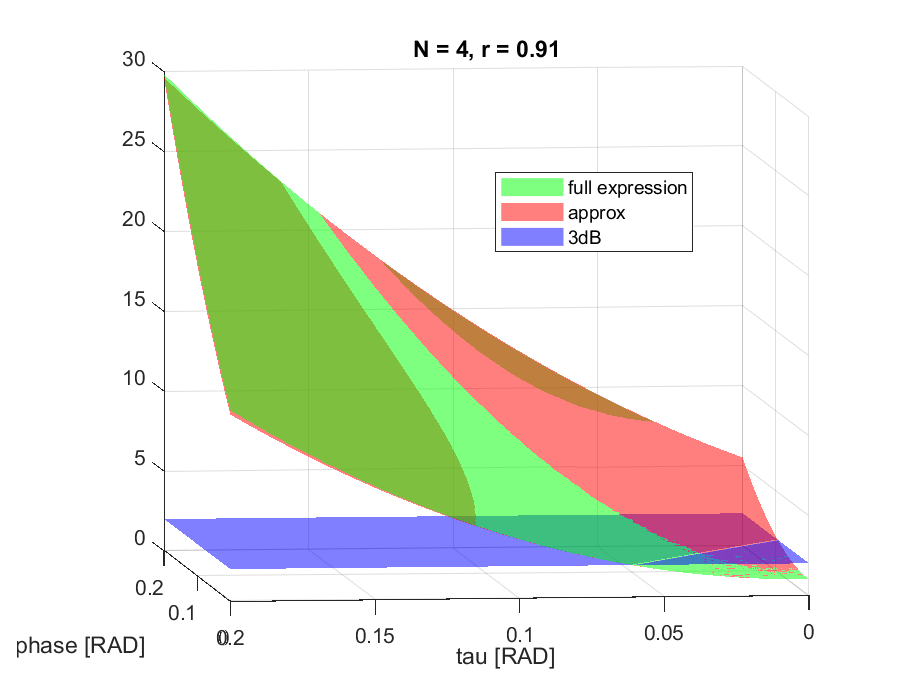
\includegraphics[width=0.9\linewidth]{./Media/spatial_IIR_MATLAB/beamwidth/BW_approx_validation.eps}
    \caption{Graphically comparing (\ref{eqn_arrayPerformance_beamwidth_fullEpxr}) and (\ref{eqn_arrayPerformance_beamwidth_approx}) for $N=4$ and $\rho=0.91$. The approximation seems to closely match the original expression.}
\end{figure}
Unlike the passive ULA case, it is evident from figure (\ref{fig_singleFreqFeedback_2ndTaylorNumericalValidation}) that the $4^{th}$ order terms are not needed for the evaluation of $\theta_{HPBW}$. In perfect phase alignment (i.e. $\Delta_{\tau}=0$), the u-space expression for the HPBW is $$u_{HPBW} =
\frac{
\left|1-\rho\right|
}{
\pi{d}
}
\lambda
\sqrt{\frac{
12
}{
\left(N-1\right)\left(\left(1+2r\right)N-4r+1\right)
}}.
$$
Comparing to the classic ULA beamwidth \cite{VanTrees2002DetectionIV}, thoroughly discussed in appendix \ref{appendix_theULABeamwidth}, we can express the improvement factor as
$$
\frac{
0.89\frac{\lambda}{ND}
}{
\theta_{HPBW,IIR}
}
=
\frac{0.89}{\left|1-\rho\right|}\sqrt{\frac{1+2r}{12}}
$$
\todo{TODO}
\textbf{Add graph of the improvement factor}
% \subsection{The pole-based design approach}
% In this approach, we look for setting the response "poles" which minimize the denominator, thus maximizing the overall response magnitude. To evaluate the beamwidth, we chose to allocate all of the system's poles in a single position such that 
% $
% 1-\vecnot{\beta}^{T}\vecnot{d}_{\theta}e^{-j\tau}
% =
% \left(e^{j\theta}-re^{j\theta_{s}}\right)^{N}
% $
% where $N$ is the number of array sensors and $r \in \left[0,1\right)$ enables us to avoid treatment of $\infty$-valued expressions. Next, we look for $\theta$ such that
% $
% \left|\frac{
% \frac
% {
% \vecnot{\alpha}^{T}\vecnot{d}_{\theta_{s}}
% }{
% \vecnot{\beta}^{T}\vecnot{d}_{\theta_{s}}
% }
% }{
% \frac
% {
% \vecnot{\alpha}^{T}\vecnot{d}_{\theta}
% }{
% \vecnot{\beta}^{T}\vecnot{d}_{\theta}
% }
% }\right|
% = \frac{1}{\sqrt{2}}
% $. Assuming that, like in classical IIR filter design theory, the numerator behaviour is significantly "slower" than the denominator's which results in $\vecnot{\alpha}^{T}\vecnot{d}_{\theta} 
% \approx
% \vecnot{\alpha}^{T}\vecnot{d}_{\theta_{s}}$ reults in
% \begin{align*}
%     \left|\frac{
%     \vecnot{\beta}^{T}\vecnot{d}_{\theta}
%     }{
%     \vecnot{\beta}^{T}\vecnot{d}_{\theta_{s}}
%     }\right|
%     &= \frac{1}{\sqrt{2}}
%     \\
%     \left|
%     \frac{
%     \left(e^{j\theta}-re^{j\theta}\right)^{N}
%     }{
%     \left(e^{j\theta}-re^{j\theta_{s}}\right)^{N}
%     }
%     \right|
%     &=
%     \left|
%     \frac{
%     \left(1-re^{j\left(\theta_{s}-\theta\right)}\right)
%     }{
%     \left(1-r\right)
%     }
%     \right|^{N}
%     \\
%     &=
%     \left|
%     \frac{
%     1+r^{2}-2r\cos{\left(\theta_{s}-\theta\right)}
%     }{
%     \left(1-r\right)^{2}
%     }
%     \right|^{\frac{N}{2}}
%     =
%     \left(\frac{1}{2}\right)^{\frac{1}{2}}
%     \\
%     \Rightarrow 
%     1+r^{2}-2r\cos{\left(\theta_{s}-\theta\right)}
%     &=
%     \left(1-r\right)^{2}2^{\frac{1}{N}}
%     \\
%     \cos{\left(\theta_{s}-\theta\right)}
%     &=
%     \frac{
%     1+r^{2}-\left(1-r\right)^{2}2^{\frac{1}{N}}
%     }{
%     2r
%     }
%     \\
%     \Rightarrow
%     \frac{\omega{D\left(cos(\theta_{g,s})-cos(\theta_{g,B})\right)}}{c}
%     &=
%     cos^{-1}
%     \left(
%     \frac{1+r^{2}-\left(1-r\right)^{2}2^{\frac{1}{N}}}{2r}
%     \right)
% \end{align*}.
% Therefore,
% \begin{equation}
%     \theta_{g,B} 
%     &= 
%     cos^{-1}
%     \left(
%     cos(\theta_{g,s})
%     -
%     \frac{c}{\omega{D}}
%     cos^{-1}
%     \left(
%     \frac{1+r^{2}-\left(1-r\right)^{2}2^{\frac{1}{N}}}{2r}
%     \right)
%     \right)
% \end{equation}
% Few observations can be derived from the $ \theta_{g,B} $:
% \begin{itemize}
%     \item $r\rightarrow{1}$ (i.e. setting the pole on the unit circle) causes $\theta_{g,B}\rightarrow\theta_{g,s}$ due to the $\infty$ valued response at $\theta_{g,s}$
%     \item The interval 
%     $
%     \left\{
%     \theta_{g,s}
%     \ \Bigg{|}\ 
%     cos(\theta_{g,s})
%     -
%     \frac{c}{\omega{D}}
%     cos^{-1}
%     \left(
%     \frac{1+r^{2}-\left(1-r\right)^{2}2^{\frac{1}{N}}}{2r}
%     \right)
%     <-1
%     \right\}
%     $, has no solution. In simulations, when evaluating such $\theta_{g,s}$ values, one can observe that the actual beampattern does not resemble the designed one due to the ULA geometric properties.
%     \item The number of sensors $N$ seems to have low impact on the beamwidth.
% \end{itemize}
% An example of a floating figure using the graphicx package.
% Note that \label must occur AFTER (or within) \caption.
% For figures, \caption should occur after the \includd to preserve the operation of \label within \caption
% even when the captionsoff option is in effect. However, because
% of issues like this, it may be the safest practice to put all your
% \label just afegraphics.
% Note that IEEEtran v1.7 and later has special internal code that
% is designeter \caption rather than within \caption{}.
%
% Reminder: the "draftcls" or "draftclsnofoot", not "draft", class
% option should be used if it is desired that the figures are to be
% displayed while in draft mode.
%
%\begin{figure}[!t]
%\centering
%\includegraphics[width=2.5in]{myfigure}
% where an .eps filename suffix will be assumed under latex, 
% and a .pdf suffix will be assumed for pdflatex; or what has been declared
% via \DeclareGraphicsExtensions.
%\caption{Simulation results for the network.}
%\label{fig_sim}
%\end{figure}
% Note that the IEEE typically puts floats only at the top, even when this
% results in a large percentage of a column being occupied by floats.
% An example of a double column floating figure using two subfigures.
% (The subfig.sty package must be loaded for this to work.)
% The subfigure \label commands are set within each subfloat command,
% and the \label for the overall figure must come after \caption.
% \hfil is used as a separator to get equal spacing.
% Watch out that the combined width of all the subfigures on a 
% line do not exceed the text width or a line break will occur.
%
%\begin{figure*}[!t]
%\centering
%\subfloat[Case I]{\includegraphics[width=2.5in]{box}%
%\label{fig_first_case}}
%\hfil
%\subfloat[Case II]{\includegraphics[width=2.5in]{box}%
%\label{fig_second_case}}
%\caption{Simulation results for the network.}
%\label{fig_sim}
%\end{figure*}
%
% Note that often IEEE papers with subfigures do not employ subfigure
% captions (using the optional argument to \subfloat[]), but instead will
% reference/describe all of them (a), (b), etc., within the main caption.
% Be aware that for subfig.sty to generate the (a), (b), etc., subfigure
% labels, the optional argument to \subfloat must be present. If a
% subcaption is not desired, just leave its contents blank,
% e.g., \subfloat[].
% An example of a floating table. Note that, for IEEE style tables, the
% \caption command should come BEFORE the table and, given that table
% captions serve much like titles, are usually capitalized except for words
% such as a, an, and, as, at, but, by, for, in, nor, of, on, or, the, to
% and up, which are usually not capitalized unless they are the first or
% last word of the caption. Table text will default to \footnotesize as
% the IEEE normally uses this smaller font for tables.
% The \label must come after \caption as always.
%
%\begin{table}[!t]
%% increase table row spacing, adjust to taste
%\renewcommand{\arraystretch}{1.3}
% if using array.sty, it might be a good idea to tweak the value of
% \extrarowheight as needed to properly center the text within the cells
%\caption{An Example of a Table}
%\label{table_example}
%\centering
%% Some packages, such as MDW tools, offer better commands for making tables
%% than the plain LaTeX2e tabular which is used here.
%\begin{tabular}{|c||c|}
%\hline
%One & Two\\
%\hline
%Three & Four\\
%\hline
%\end{tabular}
%\end{table}
% Note that the IEEE does not put floats in the very first column
% - or typically anywhere on the first page for that matter. Also,
% in-text middle ("here") positioning is typically not used, but it
% is allowed and encouraged for Computer Society conferences (but
% not Computer Society journals). Most IEEE journals/conferences use
% top floats exclusively. 
% Note that, LaTeX2e, unlike IEEE journals/conferences, places
% footnotes above bottom floats. This can be corrected via the
% \fnbelowfloat command of the stfloats package.
\section{Conclusions}
\label{sec_conclusions}
In this contribution we have presented a novel concept of spatial feedback-based beamforming. In the context of ULA, this approach can be seen as extension of FIR filtering, to IIR filter design, for spatial localization.
\par We have analyzed and shown that the feedback-beamformer is superior to the conventional delay and sum beamformer, achieving improved beamwidth, sidelobe attenuation and directivity.
\par The suggested approach revealed itself to be sensitive to target range errors. Hence, we have suggested to mitigate this sensitivity by transmitting with two  independent and closely spaced frequencies.
\par This paper lays the ground for a diverse future research, starting from different approaches of setting the beamformer weights $\vAlpha,\vBeta$, waveform design, localization performance analysis, extension to moving targets and generalization to multiple-input-multiple-output (MIMO) systems.
% if have a single appendix:
%\appendix[Proof of the Zonklar Equations]
% or
%\appendix  % for no appendix heading
% do not use \section anymore after \appendix, only \section*
% is possibly needed

% use appendices with more than one appendix
% then use \section to start each appendix
% you must declare a \section before using any
% \subsection or using \label (\appendices by itself
% starts a section numbered zero.)
%
\appendices
\section{FIM calculation}
\label{apdx_clacFim}
Following \eqref{eq_beamPatternFreqDomain_FIM}, we elaborate the steps leading to \eqref{eqn_FIMelements}. First, we express the parial derivatives of $\F{y}$ with respect to $\vEta$, resulting in
\begin{equation*}
    \resizebox{.9\linewidth}{!}{
        \begin{split}
            \frac{\partial{\F{y}}}{\partial{\thetaD}} &= 
            \frac{
            \vBetaT{}A\omegaB\vd\ePhi{-}\rBrace{1-\aTd\ePhi{-}}+\bTd\vAlphaT{}A\omegaB\vd\ePhi{-2}
            }{
            \rBrace{1-\aTd\ePhi{-}}^{2}
            }
            \\&=
            \frac{
            \vBetaT{}A\omegaB\vd\ePhi{-}-\vBetaT{}\rBrace{A\omegaB\vd\vdT-\vd\vdT{}A\omegaB}\vAlpha\ePhi{-2}
            }{
            \rBrace{1-\aTd\ePhi{-}}^{2}
            }
            \\&=
            \frac{
            \vBetaT{}A\omegaB\vd\ePhi{-}-\vBetaT{}B\omegaB\vAlpha\ePhi{-2}
            }{
            \rBrace{1-\aTd\ePhi{-}}^{2}
            }
        \end{split}
    }
\end{equation*}
and
\begin{equation*}
    \resizebox{.9\linewidth}{!}{
        \begin{split}
            \frac{\partial{\F{y}}}{\partial{\phi}} &= 
            \frac{
            -j\bTd\ePhi{-}\rBrace{1-\aTd\ePhi{-}}-j\bTd\aTd\ePhi{-2}
            }{
            \rBrace{1-\aTd\ePhi{-}}^{2}
            }
            \\&=
            \frac{
            -j\bTd\ePhi{-}
            }{
            \rBrace{1-\aTd\ePhi{-}}^{2}
            }
        \end{split}
    }
\end{equation*}
such that
\begin{equation*}
    \resizebox{.9\linewidth}{!}{
        \begin{split}
            J_{\thetaD\thetaD} &= \Re\cBrace{\frac{1}{2\pi\sigma^{2}}\int_{-\omega_{s}/2}^{\omega_{s}/2}\lBrace{\frac{\partial{\F{y}\omegaB}}{\partial{\thetaD}}}^{2}d\omega}
            \\&=
            \frac{1}{2\pi\sigma^{2}}\int_{-\omega_{s}/2}^{\omega_{s}/2}{\frac{
            \lBrace{\vBetaT{}A\omegaB\vd-\vBetaT{}B\omegaB\vAlpha\ePhi{-}}^{2}
            }{
            \lBrace{1-\aTd\ePhi{-}}^{4}
            }\lBrace{\F{x}\omegaB}^{2}d\omega},
            \\
            J_{\phi\phi} &= \Re\cBrace{\frac{1}{2\pi\sigma^{2}}\int_{-\omega_{s}/2}^{\omega_{s}/2}\lBrace{\frac{\partial{\F{y}\omegaB}}{\partial{\phi}}}^{2}d\omega}
            \\&=
            \frac{1}{2\pi\sigma^{2}}\int_{-\omega_{s}/2}^{\omega_{s}/2}{\frac{
            \lBrace{\bTd}^{2}
            }{
            \lBrace{1-\aTd\ePhi{-}}^{4}
            }\lBrace{\F{x}\omegaB}^{2}d\omega}
        \end{split}
    }
\end{equation*}
and the cross terms are
\begin{equation*}
    \resizebox{.9\linewidth}{!}{
        \begin{split}
            &J_{\thetaD\phi} = J_{\phi\thetaD}^{\ast} = 
            \\&= \Re\cBrace{\frac{1}{2\pi\sigma^{2}}\int_{-\omega_{s}/2}^{\omega_{s}/2}
            \rBrace{\frac{\partial{\F{y}\omegaB}}{\partial{\phi}}}^{\ast}
            \frac{\partial{\F{y}\omegaB}}{\partial{\thetaD}}d\omega}
            \\&=
            \Re\cBrace{\frac{1}{2\pi\sigma^{2}}\int_{-\omega_{s}/2}^{\omega_{s}/2}{\frac{
            j\vBetaT{}\rBrace{A\omegaB\vd-B\omegaB\vAlpha\ePhi{-}}\vdH\vBetaC
            }{
            \lBrace{1-\aTd\ePhi{-}}^{4}
            }\lBrace{\F{x}\omegaB}^{2}d\omega}}.
        \end{split}
    }
\end{equation*}
Setting the coefficients as $$\vAlpha,\vBeta\propto\vd^{\ast}$$ causes the $\vBetaT{}B\omegaB\vAlpha$~term to vanish. Assuming real input and real gain terms $g_n$ within the steering vector, the function
\[
\frac{\lBrace{\F{x}\omegaB}^{2}}{\lBrace{1-\aTd\ePhi{-}}^{4}}
\]
is even with respect to $\omega$, and $$j\vBetaT{}A\omegaB\vd\vdH\vBetaC\propto A\omegaB\vd\norm{\vd}^2$$ is odd. Hence the cross terms vanish.

\section{Half power beamwidth}
\label{apdx_HPBW}
We now equate the squared norm of \eqref{eq_Hdphi0} to $0.5$ and compute the value of $N\dTheta/2$ for large $N$. Denoting $\gamma\triangleq\dTheta/2$,
\begin{equation*}
    \resizebox{1\linewidth}{!}{
        \begin{split}
            \abs{\Hr_{\dTheta,\dPhi=0,r}\rBrace{\omega}}^{2}&=
             \frac{\rBrace{1-r}^{2}\Dp{\gamma,N}{2}}{\abs{\exp\rBrace{j(N-1)\gamma}-r\D{\gamma}{N}}^{2}}
             \\&
             \overset{N\gg1}{\approx}\frac{\rBrace{1-r}^{2}\Dp{\gamma,N}{2}}{1-2r\cos{\rBrace{N\gamma}}\D{\gamma}{N}+r^{2}\Dp{\gamma,N}{2}}\overset{!}{=}\frac{1}{2},
        \end{split}
    }
\end{equation*}
which leads to 
\begin{equation*}
    % \resizebox{1\linewidth}{!}{
        \begin{split}
            \rBrace{r^{2}-4r+2}\Dp{\gamma,N}{2}+2r\cos{\rBrace{N\gamma}}\D{\gamma}{N}-1 = 0.
        \end{split}
    % }
\end{equation*}
Since for large $N$, the main lobe width goes to zero, we approximating $\sin(\gamma)$ with $\gamma$. Also defining $x\triangleq{}N\gamma=N\dTheta/2$ we obtain \eqref{eq_HPBW}.

% \section{The ULA beamwidth}
% \label{appendix_theULABeamwidth}
% Following \cite{VanTrees2002DetectionIV}'s half power beam width (HPBW) calculation steps assuming classic passive ULA under the conventional beamformer, we start at equation (2.96) which express the beampattern in $u$-space, stating that
$$
B_{u}\left(u\right)=
\frac{1}{N}
\frac{
sin\left(\frac{\pi{}Nd}{\lambda}u\right)
}{
sin\left(\frac{\pi{}d}{\lambda}u\right)
}.
$$
In this paper, we define $\dTheta = \frac{2\pi{}d\left(\cos\left(\theta_{g}\right)-\cos\left(\theta_{g,s}\right)\right)}{\lambda}$, therefore
$$
B_{\theta_{g}}\left(\theta_{g}\right)=
\frac{1}{N}
\frac{
\sin\left(N\dTheta\right)
}{
\sin\left(\dTheta\right)
},
$$
i.e.
\begin{equation}
     u = 2\cos\left(\theta_{g}\right).
\end{equation}
Comparing $B_{u}\left(u\right)$ to $1/\sqrt{2}$ for the extraction of $u_{HPBW}$, \cite{VanTrees2002DetectionIV} determines (equation 2.98) that the HPBW is achieved by setting 
\begin{equation}
    \label{eqn_classicULA_beamwidthCalc_VanTrees_eq_2_98}
    \frac{\pi{}Nd}{\lambda}u = 1.4
\end{equation}
and hints in the matching problem (2.4.7) that the number $1.4$ can be calculated using the $2^{nd}$ order taylor expansion of $B_{u}\left(u\right)$. Equivalent analysis of $ f_{N}\left(x\right)\triangleq\frac{\sin\left(Nx\right)}{\sin\left(x\right)} $ and expansion to its second order terms (i.e.
$
\evalat{f\left(x\right)}{x\to{}a,} \approx 
f(a) + 
\frac{1}{1!}\evalat{\frac{\partial{f}}{\partial{x}}}{\left(x=a\right)}\left(x-a\right) 
+ 
\frac{1}{2!}\evalat{\frac{\partial{f}}{\partial{x^{2}}}}{\left(x=a\right)}\left(x-a\right)^{2}
$), results in
\begin{equation}
    \evalat{f\left(x\right)}{x\to0}
    \approx
    1 + \frac{1}{2!}\left(\frac{N^{2}-1}{3}\right)x^{2}.
\end{equation}
Comparing to $1/\sqrt{2}$, one can write
\begin{equation*}
    Nx_{HPBW} = N\sqrt{\frac{6\left(1-1/\sqrt{2}\right)}{N^{2}-1}}
    \overset{N>>1}{\to} \sqrt{6\left(1-1/\sqrt{2}\right)} \approx 1.325,
\end{equation*}
which doesn't quite fit the stated value (\ref{eqn_classicULA_beamwidthCalc_VanTrees_eq_2_98}). This lead us to investigate a higher order taylor expansions. As can be verified, $\evalat{\frac{\partial{f}}{\partial{x}^{3}}}{x=0} = 0$, leading to expressing the $4^{th}$ order term
\begin{equation}
    \evalat{f\left(x\right)}{x\to0}
    \approx
    1 
    + 
    \frac{1}{2!}\left(\frac{N^{2}-1}{3}\right)x^{2}
    +
    \frac{1}{4!}\left(\frac{N^{4}}{10}-\frac{2N^{2}}{6}+\frac{1}{15}\right)x^{4}
\end{equation}
which conveniently generates a quadratic equation with respect to $x^{2}$. We plot $Nx_{HPBW}$ for various values of $N$ in fig.(\ref{fig_classicULA_beamwidth_Nx_HPBW}) and one can see that indeed, as stated in \cite{VanTrees2002DetectionIV}, $Nx_{HPBW}$ tends toward $1.4$ as $N$ increases.
\begin{figure}
    \label{fig_classicULA_beamwidth_Nx_HPBW}
    \centering
    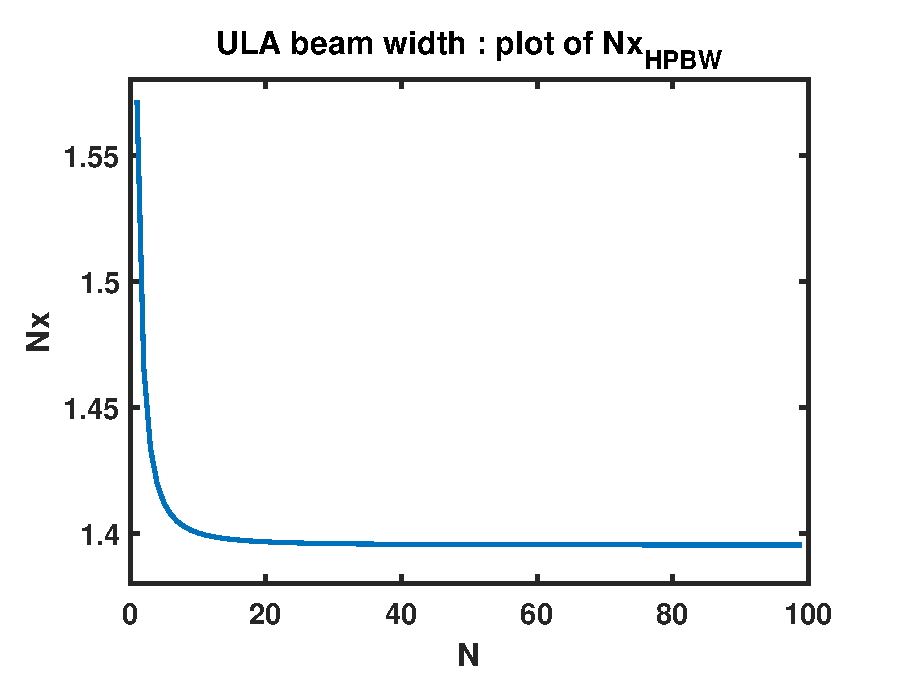
\includegraphics[width=0.6\linewidth]{./Media/spatial_IIR_MATLAB/beamwidth/Nx_HPBW.eps}
    \caption{Plot of $Nx_{HPBW}$ for various $N$ values. For each $N$, $x_{HPBW}$ was calculated as a solution to the quadratic equation (with respect to $x^{2}$) and mutiplied by the matching $N$. Although $x_{HPBW}$ monotonically decreasing as $N$ increases, it is evident that $Nx_{HPBW}$ tends towards a finite limit of $\sim1.4$.}
\end{figure}
With \cite{VanTrees2002DetectionIV}'s equation (2.96) (\ref{eqn_classicULA_beamwidthCalc_VanTrees_eq_2_98} in our paper) proven, using the fact that $u = 2\cos{\theta_{g}}$ (where $\theta_{g}$ is the geometric angle), one can write that
$$
u_{HPBW} = \frac{\lambda}{Nd}\frac{1.4}{\pi}.
$$
Therefore, considering that $B_{u}\left(u\right)$ is an even function, the actual beamwidth is twice the size of $u_{HPBW}$ 
\begin{equation}
    HPBW_{u} = 2u_{HPBW} = \frac{2.8}{\pi}\frac{\lambda}{Nd} \approx 0.891\frac{\lambda}{Nd}
\end{equation}
as stated in \cite{VanTrees2002DetectionIV}'s equation (2.100). For other spaces representation of the HPBW, see \cite{VanTrees2002DetectionIV}'s (table 2.2), where for the $\theta_{g}$-space, $\Tilde{\theta_{g}} \triangleq \pi/2-\theta_{g}$ was defined to emphasize that the entire analysis of the beampattern was under the assumption that $\theta_{g,s}=\pi/2$, stating that
\begin{equation}
    \Tilde{\theta}_{g,HPBW} = 2\sin^{-1}\left(0.446\frac{\lambda}{Nd}\right)
\end{equation}
and for small $\Tilde{\theta}_{g}$ (i.e large $N$ values),
\begin{equation}
    \Tilde{\theta}_{g,HPBW} \approx 0.891\frac{\lambda}{Nd}
\end{equation}
% you can choose not to have a title for an appendix
% if you want by leaving the argument blank
% use section* for acknowledgment
\section*{Acknowledgment}

The authors would like to thank...


% Can use something like this to put references on a page
% by themselves when using endfloat and the captionsoff option.
\ifCLASSOPTIONcaptionsoff
  \newpage
\fi



% trigger a \newpage just before the given reference
% number - used to balance the columns on the last page
% adjust value as needed - may need to be readjusted if
% the document is modified later
%\IEEEtriggeratref{8}
% The "triggered" command can be changed if desired:
%\IEEEtriggercmd{\enlargethispage{-5in}}

% references section

% can use a bibliography generated by BibTeX as a .bbl file
% BibTeX documentation can be easily obtained at:
% http://mirror.ctan.org/biblio/bibtex/contrib/doc/
% The IEEEtran BibTeX style support page is at:
% http://www.michaelshell.org/tex/ieeetran/bibtex/
\bibliographystyle{IEEEtran}
\bibliography{./Modules/Mendeley,./Modules/LocalBib}% ./Modules/LocalBib}
% argument is your BibTeX string definitions and bibliography database(s)
% \bibliography{IEEEabrv,../bib/paper}
%
% <OR> manually copy in the resultant .bbl file
% set second argument of \begin to the number of references
% (used to reserve space for the reference number labels box)
% \begin{thebibliography}{1}

% \bibitem{IEEEhowto:kopka}
% H.~Kopka and P.~W. Daly, \emph{A Guide to \LaTeX}, 3rd~ed.\hskip 1em plus
%   0.5em minus 0.4em\relax Harlow, England: Addison-Wesley, 1999.

% \end{thebibliography}

% biography section
% 
% If you have an EPS/PDF photo (graphicx package needed) extra braces are
% needed around the contents of the optional argument to biography to prevent
% the LaTeX parser from getting confused when it sees the complicated
% \includegraphics command within an optional argument. (You could create
% your own custom macro containing the \includegraphics command to make things
% simpler here.)
%\begin{IEEEbiography}[{\includegraphics[width=1in,height=1.25in,clip,keepaspectratio]{mshell}}]{Michael Shell}
% or if you just want to reserve a space for a photo:

\begin{IEEEbiography}[{\includegraphics[width=1in,height=1.25in,clip,keepaspectratio]{./Media/addPhotoHere.PNG}}]{Israel Cohen}
(M’01–SM’03–F’15) He received the B.Sc. (Summa Cum Laude), M.Sc., and Ph.D. degrees in electrical engineering from the Technion – Israel Institute of Technology, Haifa, Israel, in 1990, 1993, and 1998, respectively.
He is currently a Professor of electrical engineering with the Technion – Israel Institute of Technology.
From 1990 to 1998, he was a Research Scientist with RAFAEL Research Laboratories, Israel Ministry of Defense, Haifa. 
From 1998 to 2001, he was a Postdoctoral Research Associate with the Computer Science Department, Yale University, New Haven, CT, USA. In 2001, he joined the Electrical Engineering Department, Technion – Israel Institute of Technology.
He is a coeditor of the Multichannel Speech Processing Section of the Springer Handbook of Speech Processing (Springer, 2008), and a coauthor of Fundamentals of Signal Enhancement and Array Signal Processing (Wiley-IEEE Press, 2017). 
His research interests include array processing, statistical signal processing, analysis and modeling of acoustic signals, speech enhancement, noise estimation, microphone arrays, source localization, blind source separation, system identification, and adaptive filtering.
Dr. Cohen was awarded the Norman Seiden Prize for Academic Excellence (2017), the SPS Signal Processing Letters Best Paper Award (2014), the Alexander Goldberg Prize for Excellence in Research (2010), and the Muriel and David Jacknow Award for Excellence in Teaching (2009). 
He is currently an Associate Member of the IEEE Audio and Acoustic Signal Processing Technical Committee. 
He was an Associate Editor for the IEEE TRANSACTIONS ON AUDIO, SPEECH, AND LANGUAGE PROCESSING and the IEEE SIGNAL PROCESSING LETTERS, and as Member of the IEEE Audio and Acoustic Signal Processing
Technical Committee and the IEEE Speech and Language Processing Technical Committee.
\end{IEEEbiography}

% if you will not have a photo at all:
\begin{IEEEbiography}[{\includegraphics[width=1in,height=1.25in,clip,keepaspectratio]{./Media/addPhotoHere.PNG}}]{Tsvi G. Dvorkind}
Tsvi G. Dvorkind received the B.Sc. degree (summa cum laude) in computer engineering in 2000, the M.Sc. degree (summa cum laude) in electrical engineering in 2003, and the Ph.D. degree in electrical engineering in 2007, all from the Technion—Israel Institute of Technology, Haifa, Israel.
From 1998 to 2000 he worked at the Electro-Optics Research & Development Company at the Technion, and during 2000–2001 at the Jigami Corporation.
He is now with the Rafael Company, Haifa, Israel.
His research interests include speech enhancement and acoustical localization, general parameter estimation problems, and sampling theory.
\end{IEEEbiography}

% insert where needed to balance the two columns on the last page with
% biographies
%\newpage

\begin{IEEEbiography}{Itay Yehezkel Karo}
Biography text here.
\end{IEEEbiography}

% You can push biographies down or up by placing
% a \vfill before or after them. The appropriate
% use of \vfill depends on what kind of text is
% on the last page and whether or not the columns
% are being equalized.

%\vfill

% Can be used to pull up biographies so that the bottom of the last one
% is flush with the other column.
%\enlargethispage{-5in}



% that's all folks
\end{document}


